\documentclass[11pt,reqno,a4letter]{article} 

\usepackage{amsmath,amssymb,amsfonts,amscd}

\usepackage{url}
\usepackage{hyperref}
\usepackage[usenames,dvipsnames]{xcolor}
\hypersetup{
    colorlinks,
    linkcolor={black!63!darkgray},
    citecolor={blue!70!white},
    urlcolor={blue!80!white}
}
\usepackage{graphicx} 

\usepackage{ocr}
\usepackage[T1]{fontenc}

\newcommand{\hlocalref}[1]{\hyperref[#1]{\ref{#1}}}

\usepackage{datetime} 
\usepackage{cancel}
\usepackage{soul} 
\usepackage{subcaption}
\captionsetup{format=hang,labelfont={bf},textfont={small,it}} 
\numberwithin{equation}{section} 
\numberwithin{figure}{section}
\numberwithin{table}{section}

\usepackage{tocloft}
\usepackage{framed} 

\usepackage{enumitem}
\setlist[itemize]{noitemsep,topsep=0pt,leftmargin=0.23in,label={\tiny$\blacksquare$}}

\usepackage{changepage}
\usepackage{rotating,adjustbox}
\usepackage{bigints}

\usepackage{diagbox}
\newcommand{\trianglenk}[2]{$\diagbox{#1}{#2}$}
\newcommand{\trianglenkII}[2]{\diagbox{#1}{#2}}

\let\citep\cite

\newcommand{\undersetbrace}[2]{\underset{\displaystyle{#1}}{\underbrace{#2}}}

\newcommand{\gkpSI}[2]{\ensuremath{\genfrac{\lbrack}{\rbrack}{0pt}{}{#1}{#2}}} 
\newcommand{\gkpSII}[2]{\ensuremath{\genfrac{\lbrace}{\rbrace}{0pt}{}{#1}{#2}}}
\newcommand{\cf}{cf.~} 
\newcommand{\Iverson}[1]{\ensuremath{\left[#1\right]_{\delta}}} 
\newcommand{\floor}[1]{\left\lfloor #1 \right\rfloor} 
\newcommand{\ceiling}[1]{\left\lceil #1 \right\rceil} 
\newcommand{\e}[1]{e\left(#1\right)} 
\newcommand{\seqnum}[1]{\href{http://oeis.org/#1}{\color{ProcessBlue}{\underline{#1}}}}

\usepackage{upgreek,dsfont,amssymb}
\renewcommand{\chi}{\upchi}
\newcommand{\ChiFunc}[1]{\ensuremath{\chi_{\{#1\}}}}
\newcommand{\OneFunc}[1]{\ensuremath{\mathds{1}_{#1}}}

%\usepackage{mathabx}
\makeatletter
\newcommand*\rel@kern[1]{\kern#1\dimexpr\macc@kerna}
\newcommand*\widebar[1]{%
  \begingroup
  \def\mathaccent##1##2{%
    \rel@kern{0.8}%
    \overline{\rel@kern{-0.8}\macc@nucleus\rel@kern{0.2}}%
    \rel@kern{-0.2}%
  }%
  \macc@depth\@ne
  \let\math@bgroup\@empty \let\math@egroup\macc@set@skewchar
  \mathsurround\z@ \frozen@everymath{\mathgroup\macc@group\relax}%
  \macc@set@skewchar\relax
  \let\mathaccentV\macc@nested@a
  \macc@nested@a\relax111{#1}%
  \endgroup
}

\usepackage{MnSymbol}
\newcommand{\gkpEII}[2]{\ensuremath{\genfrac{\llangle}{\rrangle}{0pt}{}{#1}{#2}}}

\usepackage{ifthen}
\newcommand{\Hn}[2]{
     \ifthenelse{\equal{#2}{1}}{H_{#1}}{H_{#1}^{\left(#2\right)}}
}

\newcommand{\Floor}[2]{\ensuremath{\left\lfloor \frac{#1}{#2} \right\rfloor}}
\newcommand{\Ceiling}[2]{\ensuremath{\left\lceil \frac{#1}{#2} \right\rceil}}

\DeclareMathOperator{\DGF}{DGF} 
\DeclareMathOperator{\ds}{ds} 
\DeclareMathOperator{\Id}{Id}
\DeclareMathOperator{\fg}{fg}
\DeclareMathOperator{\Div}{div}
\DeclareMathOperator{\rpp}{rpp}
\DeclareMathOperator{\logll}{\ell\ell}

\title{
       Exact formulas for partial sums of the M\"obius function expressed by 
       partial sums weighted by the Liouville lambda function
}
\author{Maxie Dion Schmidt \\
        {\normalsize \href{mailto:maxieds@gmail.com}{maxieds@gmail.com}} \\
        Georgia Institute of Technology \\
        School of Mathematics
}  
\date{\small\underline{Last Revised:} \today \ @\ \hhmmsstime{} \ -- \ Compiled with \LaTeX2e} 

\usepackage{amsthm} 

\theoremstyle{plain} 
\newtheorem{theorem}{Theorem}
\newtheorem{conjecture}[theorem]{Conjecture}
\newtheorem{claim}[theorem]{Claim}
\newtheorem{prop}[theorem]{Proposition}
\newtheorem{lemma}[theorem]{Lemma}
\newtheorem{cor}[theorem]{Corollary}
\numberwithin{theorem}{section}
\newtheorem*{theorem*}{Theorem}
\newtheorem*{conjecture*}{Conjecture}

\theoremstyle{definition} 
\newtheorem{example}[theorem]{Example}
\newtheorem{remark}[theorem]{Remark}
\newtheorem{definition}[theorem]{Definition}
\newtheorem{notation}[theorem]{Notation}
\newtheorem{question}[theorem]{Question}
\newtheorem{discussion}[theorem]{Discussion}
\newtheorem{facts}[theorem]{Facts}
\newtheorem{summary}[theorem]{Summary}
\newtheorem{heuristic}[theorem]{Heuristic}
\newtheorem{observation}[theorem]{Observation}
\newtheorem{ansatz}[theorem]{Ansatz}

\usepackage[compact]{titlesec}
\renewcommand{\arraystretch}{1.25} 
\newcommand{\ManuscriptMarginSize}{0.75in}
\usepackage[total={7in, 9.5in},left=\ManuscriptMarginSize,right=\ManuscriptMarginSize,
	    tmargin=\ManuscriptMarginSize,bmargin=\ManuscriptMarginSize,headsep=0pt]{geometry}
\newcommand{\PlotFigureHorizontalScalingFactor}{0.8}

\setlength{\parindent}{0em}
\setlength{\parskip}{0.5em} 

\renewcommand{\Re}{\operatorname{Re}}
\renewcommand{\Im}{\operatorname{Im}}

\newcommand{\mathtext}[1]{\text{\rm #1}}

\usepackage{tikz}
\usetikzlibrary{shapes,arrows}

\usepackage{longtable}
\usepackage{arydshln} 
\usepackage[symbols,nogroupskip,nomain,automake=true,nonumberlist,section=section]{glossaries-extra}
\usepackage{glossary-mcols} 

\defglsdisplayfirst[main]{#1#4\protect\footnote{#2}}

%%%%%%%%%%%%

\providecommand{\glossarytoctitle}{\glossaryname}
\setlength{\glsdescwidth}{0.7\textwidth}

\newglossarystyle{glossstyleSymbol}{%
\renewenvironment{theglossary}%
 {\begin{longtable}{lp{\glsdescwidth}}}%
 {\end{longtable}}%
 \setlength{\parskip}{3.5pt}
 \renewcommand{\glsgroupskip}{}
\renewcommand*\glspostdescription{\dotfill}
\renewcommand*{\glossaryheader}{%
 \bfseries Symbols & \bfseries Definition
 \\\endhead}%
 \renewcommand*{\glsgroupheading}[1]{}%
  \renewcommand{\glossentry}[2]{%
    \glstarget{##1}{\glossentrysymbol{##1}} &
    \glossentrydesc{##1} \tabularnewline
  }%
  \renewcommand*{\glspostdescription}{}
  \renewcommand{\glossarymark}[1]{}
}

\setglossarystyle{glossstyleSymbol}
\makeglossaries

%%%%%%%%%%%%

\newglossaryentry{fCvlg}{
    symbol={\ensuremath{f \ast g}},
    sort={fg},
    description={The Dirichlet convolution of any two arithmetic functions 
    $f$ and $g$ at $n$ is defined to be 
    the divisor sum $(f \ast g)(n) := \sum\limits_{d|n} f(d) g\left(\frac{n}{d}\right)$ 
    for $n \geq 1$. 
    },
    type={symbols},
    name={Dirichlet convolution}
    }
\newglossaryentry{MoebiusMuFunc}{
    symbol={\ensuremath{\mu(n),M(x)}},
    sort={MoebiusMuFunc},
    description={The M\"obius function defined such that $\mu^2(n)$ is the indicator function of the 
                 squarefree integers $n \geq 1$ where 
                 $\mu(n) = (-1)^{\omega(n)}$ whenever $n$ is squarefree. 
                 The Mertens function is the summatory function defined for all integers 
                 $x \geq 1$ by the partial sums $M(x) := \sum\limits_{n \leq x} \mu(n)$.
                 },
    type={symbols},
    name={M\"obius function}
    }
\newglossaryentry{Iverson}{
    symbol={\ensuremath{\Iverson{n=k}},\ensuremath{\Iverson{\mathtt{cond}}}},
    sort={Iverson},
    description={The symbol $\Iverson{n=k}$ is a synonym for $\delta_{n,k}$ 
                 which is one if and only if $n = k$, and is zero otherwise. 
                 For Boolean-valued conditions, \texttt{cond}, the symbol $\Iverson{\mathtt{cond}}$ 
                 evaluates to one precisely when \texttt{cond} is true or to zero otherwise.},
    type={symbols},
    name={Iverson's convention}
    }
\newglossaryentry{epsilonN}{
    symbol={\ensuremath{\varepsilon(n)}},
    sort={epsilonN},
    description={The multiplicative identity with respect to Dirichlet convolution, $\varepsilon(n) := \delta_{n,1}$, 
                 defined such that for any arithmetic function $f$ we have that 
                 $f \ast \varepsilon = \varepsilon \ast f = f$ where the operation 
                 $\ast$ denotes Dirichlet convolution. },
    type={symbols},
    name={Dirichlet multiplicative identity}
    }
\newglossaryentry{Zetas}{
    symbol={\ensuremath{\zeta(s)}},
    sort={Zetas},
    description={The Riemann zeta function is defined by 
                 $\zeta(s) := \sum\limits_{n \geq 1} n^{-s}$ when $\Re(s) > 1$, 
                 and by analytic continuation to any $s \in \mathbb{C}$ with the exception of a 
                 simple pole at $s = 1$ of residue one.},
    type={symbols},
    name={Riemann zeta function}
    }
\newglossaryentry{fInvn}{
     symbol={\ensuremath{f^{-1}(n)}},
    sort={fInvn},
    description={
     The Dirichlet inverse $f^{-1}$ of an arithmetic function $f$ exists 
     if and only if $f(1) \neq 0$. 
     The Dirichlet inverse of any $f$ such that $f(1) \neq 0$ 
     is defined recursively by 
     $f^{-1}(n) = -\frac{1}{f(1)} \times \sum\limits_{\substack{d|n \\ d>1}} f(d) f^{-1}\left(\frac{n}{d}\right)$ 
     for $n \geq 2$ with $f^{-1}(1) = f(1)^{-1}$. 
     When it exists, this inverse function 
     is unique and satisfies  $f^{-1} \ast f = f \ast f^{-1} = \varepsilon$.},
    type={symbols},
    name={Dirichlet inverse of $f$}
    }
\newglossaryentry{CkngInvAuxFunc}{
    symbol={$C_k(n),C_{\Omega}(n)$},
    sort={CkngInvAuxFunc},
    description={The first sequence is defined recursively for integers $n \geq 1$ and $k \geq 0$ as follows: 
                 \[
                 C_k(n) := \begin{cases} 
                      \delta_{n,1}, & \mathtext{ if $k = 0$; } \\ 
                      \sum\limits_{d|n} \omega(d) C_{k-1}\left(\frac{n}{d}\right), & \text{ if $k \geq 1$. } 
                      \end{cases} 
                 \]
                 It represents the multiple ($k$-fold) convolution of the function $\omega(n)$ 
                 with itself. 
                 The function $C_{\Omega}(n) := C_{\Omega(n)}(n)$ has the DGF 
                 $(1-P(s))^{-1}$ for $\Re(s) > 1$. 
                 },
    type={symbols},
    name={Dirichlet inverse component functions}
    }
\newglossaryentry{gInvn}{
    symbol={$g(n),G(x),|G|(x)$},
    sort={gInvn},
    description={The Dirichlet inverse function, $g(n) = (\omega+1)^{-1}(n)$, has the 
                 summatory function $G(x) := \sum\limits_{n \leq x} g(n)$ for $x \geq 1$. 
                 We define the partial sums of the unsigned inverse function to be 
                 $|G|(x) := \sum_{n \leq x} |g(n)|$ for $x \geq 1$. },
    type={symbols},
    name={Key Dirichlet inverse functions}
    }
\newglossaryentry{PikPiHatkx}{
    symbol={$\pi_k(x),\widehat{\pi}_k(x)$},
    sort={PikPiHatkx},
    description={For integers $k \geq 1$, the 
                 function $\pi_k(x)$ denotes the number of 
                 $2 \leq n \leq x$ with 
                 exactly $k$ distinct prime factors: $\pi_k(x) := \#\{2 \leq n \leq x: \omega(n) = k\}$. 
                 Similarly, the function 
                 $\widehat{\pi}_k(x) := \#\{2 \leq n \leq x: \Omega(n) = k\}$ for $x \geq 2$ and fixed $k \geq 1$. 
		},
    type={symbols},
    name={Distinct prime counting functions}
    }   
\newglossaryentry{primeOmegaFunctions}{
    symbol={$\omega(n)$,$\Omega(n)$}, 
    sort={OmegaPrimeOmegaFunctions},
    description={We define the strongly additive function 
                 $\omega(n) := \sum\limits_{p|n} 1$ and the completely additive function 
                 $\Omega(n) := \sum\limits_{p^{\alpha} || n} \alpha$. This means that if the prime 
                 factorization of any $n \geq 2$ is 
                 given by $n := p_1^{\alpha_1} \times \cdots \times p_r^{\alpha_r}$ 
                 with $p_i \neq p_j$ for all $i \neq j$, 
                 then $\omega(n) = r$ and $\Omega(n) = \alpha_1 + \cdots + \alpha_r$. 
                 We set $\omega(1) = \Omega(1) = 0$ by convention.},
    type={symbols},
    name={Prime omega functions}
    }
\newglossaryentry{LiouvilleLambdaFunc}{
     symbol={$\lambda(n), L(x)$}, 
    sort={LiouvilleLambdaFunc},
    description={The Liouville lambda function is the completely multiplicative function defined by 
                 $\lambda(n) := (-1)^{\Omega(n)}$. 
                 Its summatory function is defined by the partial sums 
                 $L(x) := \sum\limits_{n \leq x} \lambda(n)$ for $x \geq 1$. 
                 },
    type={symbols},
    name={Liouville lambda function}
    }
\newglossaryentry{QxSummatoryFunc}{
    symbol={$Q(x)$},
    sort={QxSummatoryFunc},
    description={For $x \geq 1$, we define $Q(x)$ to be the summatory function indicating the number of 
		 squarefree integers $n \leq x$. That is, $Q(x) = \sum_{n \leq x} \mu^2(n)$ for $x \geq 1$. }, 
    type={symbols},
    name={Summatory function of the squarefree integers}
    }
\newglossaryentry{AApproxSimGGLLRelations}{
    symbol={$\gg,\ll,\asymp,\sim$},
    sort={AApproxSimGGLLRelations},
    description={eqn_PiHatkx_UniformAsymptoticsStmt_from_MV_v1
                 For functions $A,B$, the notation $A \ll B$ implies that $A = O(B)$. 
                 Similarly, for $B \geq 0$ the notation $A \gg B$ implies that $B = O(A)$. 
                 When we have that $A, B \geq 0$, $A \ll B$ and $B \ll A$, we write $A \asymp B$. 
                 Two arithmetic functions $A(x), B(x)$ satisfy the relation $A \sim B$ if 
                 $\lim_{x \rightarrow \infty} \frac{A(x)}{B(x)} = 1$. },
    type={symbols},
    name={Asymptotic relation symbols}
    }
\newglossaryentry{PrimeZetaOAndIndicatorChiPrimeP}{
    symbol={$P(s),\chi_{\mathbb{P}}(n)$},
    sort={chiPrimeP},
    description={The indicator function of the primes as denoted by 
                 $\chi_{\mathbb{P}}(n)$. The function equals one if and only if 
                 $n \in \mathbb{Z}^{+}$ is prime and is defined to be 
                 zero-valued otherwise. 
                 For any $s \in \mathbb{C}$ such that $\Re(s) > 1$, 
                 we define the prime zeta function to be the 
                 Dirichlet generating function (DGF) defined by 
		 $P(s) = \sum\limits_{n \geq 1} \chi_{\mathbb{P}}(n) n^{-s}$. 
                 The function $P(s)$ has an analytic continuation to the half-plane 
                 $\Re(s) > 0$ with the exception of $s = 1$ through the formula 
                 $P(s) = \sum\limits_{k \geq 1} \frac{\mu(k)}{k} \times \log\zeta(ks)$. The DGF $P(s)$ 
                 has poles at the reciprocal of each positive integer and a natural boundary 
                 at the line $\Re(s) = 0$. },
    type={symbols},
    name={Prime set indicator function}
    }
\newglossaryentry{PiPrimeCountingFunc}{
    symbol={$\pi(x)$},
    sort={PrimeCountingFunc},
    description={The prime counting function denotes the number of primes $p \leq x$, i.e., $\pi(x) = \sum_{p \leq x} 1$.},
    type={symbols},
    name={Prime counting function}
    }
\newglossaryentry{WLambertWFunction}{
    symbol={$W(x)$},
    sort={WLambertWFunction},
    description={For $x,y \in [0, \infty)$, we write that $x = W(y)$ if and only if $xe^{x} = y$. 
                 This function denotes the principal branch of the multi-valued Lambert $W$ function 
                 taken over the non-negative reals. },
    type={symbols},
    name={Lambert $W$-Function}
    }
\newglossaryentry{GammaIncompleteGamma}{
    symbol={$\Gamma(a, z)$},
    sort={GammaIncompleteGamma},
    description={The incomplete gamma function is defined as $\Gamma(a, z) := \int_z^{\infty} t^{a-1} e^{-t} dt$ 
		 by continuation for $a \in \mathbb{R}$ and $|\operatorname{arg}(z)| < \pi$. }, 
    type={symbols},
    name={Incomplete gamma function}
    }
\newglossaryentry{NormalCDFFunc}{
    symbol={$\Phi(z)$},
    sort={NormalCDFFunc},
    description={For $z \in \mathbb{R}$, we take the cumulative density function 
                 of the standard normal distribution to be denoted by 
                 $\Phi(z) := \frac{1}{\sqrt{2\pi}} \times \int\limits_{-\infty}^{z} e^{-\frac{t^2}{2}} dt$. 
                },
    type={symbols},
    name={Asymptotic relation symbol}
    }

\glsaddall[types={symbols}]

\allowdisplaybreaks 

\begin{document} 

\maketitle

\begin{abstract} 
\noindent  
The Mertens function, $M(x) := \sum_{n \leq x} \mu(n)$, is 
defined as the summatory function of the classical M\"obius function.
The Dirichlet inverse function $g(n) := (\omega+\mathds{1})^{-1}(n)$
is defined in terms of the shifted strongly additive function $\omega(n)$ that counts the 
number of distinct prime factors of $n$ without multiplicity. 
The Dirichlet generating function (DGF) of $g(n)$ is $\zeta(s)^{-1} (1+P(s))^{-1}$ 
for $\Re(s) > 1$ where $P(s) = \sum_p p^{-s}$ is the prime zeta function. 
We study the distribution of the unsigned functions $|g(n)|$ with 
DGF $\zeta(2s)^{-1}(1-P(s))^{-1}$ 
and $C_{\Omega}(n)$ with DGF 
$(1-P(s))^{-1}$ for $\Re(s) > 1$. 
We prove formulas for the average order and variance of both 
$\log C_{\Omega}(n)$ and $\log |g(n)|$ and prove a central limit theorem 
for the distribution of their values over $n \leq x$ as $x \rightarrow \infty$. 
Discrete convolutions of the partial sums of $g(n)$ with the prime counting function 
provide new exact formulas for $M(x)$ that are sums of the Liouville function 
weighted by the unsigned summands $|g(n)|$. 

\bigskip\noindent
\textbf{Keywords and Phrases:} {\it M\"obius function; Mertens function; 
                                    Liouville lambda function; prime omega function; 
                                    Dirichlet inverse; Dirichlet generating function; 
				    prime zeta function; 
				    inversion theorem; inversion of generalized convolutions. } \\[0.05cm] 
% 11-XX	        Number theory
%    11A25  	Arithmetic functions; related numbers; inversion formulas
%    11Y70  	Values of arithmetic functions; tables
%    11-04  	Software, source code, etc. for problems pertaining to number theory
% 11Nxx		Multiplicative number theory
%    11N05  	Distribution of primes
%    11N37  	Asymptotic results on arithmetic functions
%    11N56  	Rate of growth of arithmetic functions
%    11N60  	Distribution functions associated with additive and positive multiplicative functions
%    11N64  	Other results on the distribution of values or the characterization of arithmetic functions
\textbf{Math Subject Classifications (2010):} {\it 11N37; 11A25; 11N60; and 11N64. } 
\end{abstract} 

%\textbf{TODO ... } Update the OEIS entries; \\ 
\textbf{TODO ... } \url{https://arxiv.org/abs/math/0306042} \\ 

\newpage
\renewcommand{\contentsname}{Article Index}
\setcounter{tocdepth}{2}
\tableofcontents

\newpage
\section{Introduction} 
\label{subSection_MertensMxClassical_Intro} 
\label{example_InvertingARecRelForMx_Intro}

\subsection{Definitions}

For integers $n \geq 2$, we define the strongly and 
completely additive functions, respectively, 
that count the number of prime divisors of $n$ by 
\begin{align*}
\omega(n) & = \sum_{p|n} 1, \mathtext{ and } 
     \Omega(n) = \sum_{p^{\alpha} \mid\mid n} \alpha. 
\end{align*}
We adopt the convention that the functions $\omega(1) = \Omega(1) = 0$. 
The M\"obius function is defined as the multiplicative function that serves as a 
signed indicator function of the squarefree integers in the form of 
\cite[\seqnum{A008683}]{OEIS}
\[
\mu(n) = \begin{cases} 
	1, & \text{ if $n = 1$}; \\ 
	(-1)^{\omega(n)}, & \text{ if $n \geq 2$ and $\omega(n) = \Omega(n)$ (i.e., if $n$ is squarefree);} \\ 
	0, & \text{ otherwise.}
        \end{cases}
\]
The Mertens function is defined by the partial sums 
\cite[\seqnum{A002321}]{OEIS} 
\begin{align} 
M(x) & = \sum_{n \leq x} \mu(n), \mathtext{ for } x \geq 1. 
\end{align} 
The Liouville lamda function is the completely multiplicative function 
defined for all $n \geq 1$ by $\lambda(n) := (-1)^{\Omega(n)}$ 
\cite[\seqnum{A008836}]{OEIS}. 
The partial sums of this function are defined by 
\cite[\seqnum{A002819}]{OEIS}
\begin{equation}
\label{eqn_LxSummatoryFuncDef_v1}
L(x) := \sum\limits_{n \leq x} \lambda(n), \mathtext{ for } x \geq 1. 
\end{equation}

\begin{definition}
For any arithmetic functions $f$ and $h$, we define their 
Dirichlet convolution at $n$ by the divisor sum 
\[
(f \ast h)(n) := \sum_{d|n} f(d) h\left(\frac{n}{d}\right), \mathtext{ for } n \geq 1.
\]
The arithmetic function $f$ has a unique inverse with respect to Dirichlet convolution, 
denoted by $f^{-1}$, if and only if $f(1) \neq 0$. 
When it exists, the Dirichlet inverse of $f$ satisfies 
$(f \ast f^{-1})(n) = (f^{-1} \ast f)(n) = \delta_{n,1}$. 
\end{definition}

We define the Dirichlet inverse function \cite[\seqnum{A341444}]{OEIS} 
\begin{equation}
\label{eqn_gInvn_def_v1}
g(n) := (\omega + \mathds{1})^{-1}(n), \mathtext{ for } n \geq 1. 
\end{equation}
Th inverse function in equation \eqref{eqn_gInvn_def_v1} 
is computed recursively by applying the formula \cite[\S 2.7]{APOSTOLANUMT}
\[
g(n) = \begin{cases}
	1, & \text{ if $n = 1$; } \\ 
	-\sum\limits_{\substack{d|n \\ d> 1}} \left(\omega(d) + 1\right) g\left(\frac{n}{d}\right), & 
	\text{ if $n \geq 2$. }
        \end{cases}
\]
The function $|g(n)| = \lambda(n) g(n)$ denotes the absolute value of $g(n)$ 
(see Proposition \hlocalref{prop_SignageDirInvsOfPosBddArithmeticFuncs_v1}). 
The summatory function of $g(n)$ is defined as follows 
\cite[\seqnum{A341472}]{OEIS}: 
\begin{equation}
\label{eqn_GInvx_PartialSumForms_v1} 
G(x) := \sum_{n \leq x} g(n) = \sum_{n \leq x} \lambda(n) |g(n)|, \mathtext{ for } x \geq 1. 
\end{equation} 

\subsection{Statements of the main results}

\begin{definition}
Let the partial sums of the 
Dirichlet convolution $r \ast h$ be defined by the function 
\begin{align*} 
S_{r \ast h}(x) & := \sum_{n \leq x} \sum_{d|n} r(d) h\left(\frac{n}{d}\right), 
	\mathtext{ for } x \geq 1. 
\end{align*}
\end{definition}

The next theorem is proved by matrix methods in 
Appendix \hlocalref{Section_PrelimProofs_Config}.

\begin{theorem} 
\label{theorem_SummatoryFuncsOfDirCvls} 
Let $r,h: \mathbb{Z}^{+} \rightarrow \mathbb{C}$ be any 
arithmetic functions such that $r(1) \neq 0$. 
Suppose that $R(x) := \sum_{n \leq x} r(n)$, $H(x) := \sum_{n \leq x} h(n)$, and that 
$R^{-1}(x) := \sum_{n \leq x} r^{-1}(n)$ for $x \geq 1$. 
The following formulas hold for all integers $x \geq 1$: 
\begin{align*} 
S_{r \ast h}(x) & \phantom{:}= \sum_{d=1}^x r(d) \times H\left(\Floor{x}{d}\right) \\ 
S_{r \ast h}(x) & \phantom{:}= \sum_{k=1}^{x} H(k) \times \left(R\left(\Floor{x}{k}\right) - 
     R\left(\Floor{x}{k+1}\right)\right). 
\end{align*} 
Moreover, for any $x \geq 1$ 
\begin{align*} 
H(x) & = \sum_{j=1}^{x} S_{r \ast h}(j) \times \left(R^{-1}\left(\Floor{x}{j}\right) - 
     R^{-1}\left(\Floor{x}{j+1}\right)\right) \\ 
     & = \sum_{k=1}^{x} r^{-1}(k) \times S_{r \ast h}(x). 
\end{align*} 
\end{theorem} 

For integers $x \geq 1$, the function $\pi(x) := \sum_{p \leq x} 1$ 
is the classical prime counting function 
\cite[\seqnum{A000720}]{OEIS}.
We find new exact formulas for $M(x)$ by applying 
Theorem \hlocalref{theorem_SummatoryFuncsOfDirCvls} 
to the expansion of the partial sums 
(see Remark \hlocalref{remark_MotivationForTheDefinitionOf_gn_v2}) 
\[
\pi(x) + 1 = \sum_{n \leq x} \sum_{d|n} \left(\omega(d) + 1\right) \mu\left(\frac{n}{d}\right), 
     \mathtext{ for } x \geq 1. 
\]

\begin{theorem} 
\label{prop_Mx_SBP_IntegralFormula} 
\begin{subequations}
For all $x \geq 1$ 
\begin{align} 
\label{prop_Mx_SBP_IntegralFormula_PartA} 
M(x) & = G(x) + \sum_{1 \leq k \leq x} |g(k)| \pi\left(\Floor{x}{k}\right) \lambda(k), \\ 
\label{prop_Mx_SBP_IntegralFormula_PartB} 
M(x) & = G(x) + 
     \sum_{1 \leq k \leq \frac{x}{2}} \left(
     \pi\left(\Floor{x}{k}\right) - \pi\left(\Floor{x}{k+1}\right) 
	\right) G(k), \\ 
\label{eqn_RmkInitialConnectionOfMxToGInvx_ProvedByInversion_v1} 
M(x) & = G(x) + \sum_{p \leq x} G\left(\Floor{x}{p}\right). 
\end{align} 
\end{subequations}
\end{theorem}

The auxiliary unsigned function $C_{\Omega}(n)$ studied by Fr\"oberg in 
\cite{FROBERG-1968} has an exact formula given by 
\begin{equation}
\label{eqn_proof_tag_hInvn_ExactNestedSumFormula_CombInterpetIdent_v3}
C_{\Omega}(n) = \begin{cases}
     1, & \text{if $n = 1$; } \\ 
     (\Omega(n))! \times \prod\limits_{p^{\alpha}||n} \frac{1}{\alpha!}, & \text{if $n \geq 2$. }
     \end{cases}
\end{equation} 

\begin{prop} 
\label{lemma_AbsValueOf_gInvn_FornSquareFree_v1} 
For all $n \geq 1$ 
\begin{equation} 
\label{eqn_AbsValueOf_gInvn_FornSquareFree_v1} 
|g(n)| = \sum_{d|n} \mu^2\left(\frac{n}{d}\right) C_{\Omega}(d). 
\end{equation} 
\end{prop} 

\begin{theorem} 
\label{lemma_HatCAstxSum_ExactFormulaWithError_v1} 
There is an absolute constant $B_0 > 0$ such that 
\[
\sum_{k \leq n} \log C_{\Omega}(k) = 
     B_0 n (\log\log n)(\log\log\log n) \left(1 + o(1)\right), 
     \mathtext{ as } n \rightarrow \infty. 
\] 
\end{theorem} 

\begin{definition}
For any $z \in (-\infty, \infty)$, the cumulative density function of any 
standard normal random variable is given by 
\[
\Phi(z) = \frac{1}{\sqrt{2\pi}} \times \int_{-\infty}^{z} e^{-\frac{t^2}{2}} dt. 
\]
\end{definition}

\begin{theorem}
\label{cor_CLT_VII}
For $x \geq 19$, let $\mu_x, \sigma_x := B_0 \cdot (\log\log x)(\log\log\log x)$. 
For any fixed $z > 0$ 
\begin{align*} 
\frac{1}{x} \times \#\left\{n \leq x: -z \leq |g(n)| - 
        \frac{1}{n} \times \sum_{k \leq n} |g(k)| \leq z\right\} & = 
        \Phi\left(\frac{\log\left(\frac{\pi^2 z}{6}\right) - \mu_x}{\sigma_x}\right) + o(1), 
	\mathtext{ as } x \rightarrow \infty.
\end{align*} 
\end{theorem}

\subsection{Organization of the manuscript}

The focus of the article is on the unsigned functions 
$C_{\Omega}(n)$ and $|g(n)|$. 
The new formulas for $M(x)$ given in 
Theorem \hlocalref{prop_Mx_SBP_IntegralFormula} 
provide a window from which we can view this function in terms of these 
auxiliary unsigned functions. 
The appendix organizes supplementary material on several 
topics that can be separated from the main sections of the article. 

\section{The function $C_{\Omega}(n)$} 
\label{Section_NewFormulasForgInvn_v1} 

The function $C_{\Omega}(n)$ is key to understanding the 
unsigned inverse sequence $|g(n)|$ through the formula in equation 
\eqref{eqn_AbsValueOf_gInvn_FornSquareFree_v1}. 
In this section, we define the function 
$C_{\Omega}(n)$ and explore its properties. 

\subsection{Definitions}

\begin{definition}
We define the following bivariate sequence for integers $n \geq 1$ and $k \geq 0$: 
\begin{align} 
\label{eqn_CknFuncDef_v2} 
C_k(n) := \begin{cases} 
     \varepsilon(n), & \text{ if $k = 0$; } \\ 
     \sum\limits_{d|n} \omega(d) C_{k-1}\left(\frac{n}{d}\right), & \text{ if $k \geq 1$. } 
     \end{cases} 
\end{align} 
Using the notation for iterated convolution in 
Bateman and Diamond \cite[Def.~2.3; \S 2]{ANT-BATEMAN-DIAMOND}, we have 
$C_0(n) \equiv \omega^{\ast 0}(n)$ and $C_k(n) \equiv \omega^{\ast k}(n)$ for 
integers $n, k \geq 1$. 
The special case of \eqref{eqn_CknFuncDef_v2} where 
$k := \Omega(n)$ occurs frequently in the next sections of the 
article. To avoid cumbersome notation when referring to this common function variant, we suppress the 
duplicate index $n$ by writing $C_{\Omega}(n) := C_{\Omega(n)}(n)$ \cite[\seqnum{A008480}]{OEIS}. 
\end{definition}

\begin{remark}
By recursively expanding the definition of $C_k(n)$ 
at any fixed $n \geq 2$, we see that 
we can form a chain of at most $\Omega(n)$ iterated (or nested) divisor sums by 
unfolding the definition of \eqref{eqn_CknFuncDef_v2} inductively. 
We also see that at fixed $n$, the function 
$C_k(n)$ is non-zero only possibly for 
$1 \leq k \leq \Omega(n)$ when $n \geq 2$. 
By equation \eqref{eqn_proof_tag_hInvn_ExactNestedSumFormula_CombInterpetIdent_v3} we have 
that $C_{\Omega}(n) \leq (\Omega(n))!$ for all $n \geq 1$ with 
equality precisely at the squarefree integers so that 
$(\Omega(n))! = (\omega(n))!$ if and only if $\mu^2(n) = 1$. 
\end{remark}

\subsection{Logarithmic average order and variance}
\label{subSection_AvgOrdersOfTheUnsignedSequences} 

\begin{lemma}
As $x \rightarrow \infty$
\begin{align}
\label{eqn_proof_tag_SumLogCOmegan_P0_exp_v1}
\sum_{n \leq x} \log C_{\Omega}(n) & \sim 
	\frac{6}{\pi^2} \times \sum_{k \geq 1} \#\{n \leq x: \Omega(n)=k\} \times \log(k!). 
\end{align}
\end{lemma}
\begin{proof}
Equation \eqref{eqn_proof_tag_hInvn_ExactNestedSumFormula_CombInterpetIdent_v3} shows that 
\[
\sum_{\substack{n \leq x \\ \mu^2(n)=1}} \log C_{\Omega}(n) = 
	\frac{6}{\pi^2} \times \sum_{k \geq 1} \#\{n \leq x: \Omega(n)=k\} \times \log(k!). 
\]
The key to the rest of the proof is to understand that the main term of the 
sum on the left-hand-side of the equation is obtained by summing over only 
the squarefree $n \leq x$, i.e., the $n \leq x$ such that $\mu^2(n) = 1$. 
We claim that 
\[
\sum_{k \geq 1} \sum_{\substack{n \leq x \\ \Omega(n)=k}} \log C_{\Omega}(n) \sim 
	\sum_{k \geq 1} \sum_{\substack{n \leq x \\ \mu^2(n) = 1 \\ \Omega(n)=k}} \log C_{\Omega}(n). 
\]
The function $\operatorname{rad}(n)$ is the radix (or squarefree part) of $n$ which evaluates 
to the largest squarefree factor of $n$, 
or equivalently to the product of all primes $p | n$ 
\cite[\seqnum{A007913}]{OEIS}. 
For integers $x \geq 1$ and $1 \leq k \leq \log_2(x)$, let the sets 
\[
\mathcal{S}_k\left(\{\varpi_j\}_{j=1}^k; x\right) := \left\{2 \leq n \leq x: \mu(n) = 0, \omega(n) = k, 
	\frac{n}{\operatorname{rad}(n)} = p_1^{\varpi_1} \times \cdots \times p_k^{\varpi_k}, 
	\mathtext{ $p_i \neq p_j$ prime for $1 \leq i < j \leq k$}\right\}. 
\]
Let the function 
$$\mathcal{N}_k(\varpi_1, \ldots, \varpi_k; x) := 
  \frac{\left\lvert \mathcal{S}_k\left(\{\varpi_j\}_{j=1}^k; x\right) \right\rvert}{x}.$$ 
The special case where $\{\varpi_j^{\ast}\}_{1 \leq j \leq k} \equiv \{0, 1\}$ 
(with value one of multiplicity exactly one) is denoted by 
$$\widehat{T}_k(x) := \mathcal{N}_k\left(\varpi_1^{\ast}, \ldots, \varpi_k^{\ast}; x\right).$$ 
If $2 \leq n \leq x$ is not squarefree and $n \in \mathcal{S}_k\left(\{\varpi_j\}_{j=1}^k; x\right)$, then 
we must have that $\varpi_j \geq 1$ for at least one $1 \leq j \leq k$. 
Clearly for any $k \geq 1$ 
\[
\mathcal{N}_k(\varpi_1, \ldots, \varpi_k; x) \ll \widehat{T}_k(x). 
\]
We claim that (see proof below) 
\begin{equation}
\label{eqn_ProofTag_HatTkx_LL_v2}
\widehat{T}_k(x) = o\left(\#\{n \leq x: \Omega(n)=k\}\right), 
     \mathtext{ for all } k \geq 1, \mathtext{ as } x \rightarrow \infty. 
\end{equation}
The upper bounds on the functions $\widehat{T}_k(x)$ in 
equation \eqref{eqn_ProofTag_HatTkx_LL_v2} 
show that the sum of denominator differences from 
\eqref{eqn_proof_tag_hInvn_ExactNestedSumFormula_CombInterpetIdent_v3} we subtract from the 
main term contributions from the squarefree $n \leq x$ is asymptotically insubstantial. 
That is, we have proved that as $x \rightarrow \infty$ 
\[
\sum_{\substack{n \leq x \\ \mu(n)=0}} \log C_{\Omega}(n) = 
     o\left(\sum_{\substack{n \leq x \\ \mu^2(n)=1}} \log C_{\Omega}(n)\right). 
     \qedhere
\]
\end{proof}

\begin{proof}[Proof of Equation \eqref{eqn_ProofTag_HatTkx_LL_v2}]
The bound can be proved by induction on $k \geq 1$ using the inductive hypothesis 
\[
\tag{IH}
\widehat{T}_m(x) \ll \frac{x^{1-2^{-m}}}{(\log x)^{1+2^{1-m}}}, 
	\mathtext{ for all } 1 \leq m \leq k, 
	\mathtext{ as } x \rightarrow \infty. 
\] 
We know that $\pi(x) \sim \frac{x}{\log x}$ as $x \rightarrow \infty$ 
\cite[\S 22.4]{HARDYWRIGHT}. 
The case where $k := 1$ is evaluated by explicit computation as follows: 
\begin{align*}
\widehat{T}_1(x) & = \sum_{p \leq \sqrt{x}} 1 \ll \frac{\sqrt{x}}{\log x}. 
\end{align*}
Suppose that $k \geq 1$ and that the IH holds at $k$. 
Then we have by the IH and 
H\"older's inequality with $\left(p^{-1}, q^{-1}\right) = \left(1-2^{-k}, 2^{-k}\right)$ that 
\begin{align*}
\widehat{T}_{k+1}(x) & \ll \sum_{p \leq \sqrt{x}} \widehat{T}_{k}\left(\frac{x}{p}\right) 
	\ll \frac{x^{1-2^{-k}}}{(\log x)^{1+2^{-k}}} \times 
	\left(\sum_{p \leq x} p^{-1}\right)^{1-2^{-k}} \times 
	\pi\left(\sqrt{x}\right)^{2^{-k}}, 
	\mathtext{ as } x \rightarrow \infty. 
\end{align*}
A famous theorem of Mertens stated as follows completes the proof by induction: 
$\sum_{p \leq x} p^{-1} \sim \log\log x$ as $x \rightarrow \infty$ 
\cite[\S 22.7--22.8]{HARDYWRIGHT}. 
Theorem \hlocalref{theorem_HatPi_ExtInTermsOfGz} 
combined with the previous argument shows that 
equation \eqref{eqn_ProofTag_HatTkx_LL_v2} holds for all $k \geq 1$.
\end{proof}

\begin{proof}[Proof of Theorem \hlocalref{lemma_HatCAstxSum_ExactFormulaWithError_v1}]  
We will split the full sum on the left-hand-side of 
\eqref{eqn_proof_tag_SumLogCOmegan_P0_exp_v1} into two sums, 
each over disjoint indices, that form the main and error terms, 
$L_{\Omega}(x)$ and $\widehat{L}_{\Omega}(x)$, respectively.
For $x \geq 3$, consider the following partial sums:
\begin{align*}
L_{\Omega}(x) & := 
	\sum_{\substack{n \leq x \\ \Omega(n) \leq \frac{3}{2} \log\log x}} \log C_{\Omega}(n), \\ 
\widehat{L}_{\Omega}(x) & := 
	\sum_{\substack{n \leq x \\ \Omega(n) > \frac{3}{2} \log\log x}} 
	\log C_{\Omega}(n).
\end{align*}
For any $z \geq 0$, 
Binet's formula for the log-gamma function is stated as follows 
\cite[\S 5.9(i)]{NISTHB}: 
\[
\log z! = \left(z+\frac{1}{2}\right)\log(1+z) - z + O(1). 
\]
Theorem \ref{theorem_HatPi_ExtInTermsOfGz} from the appendix, 
equation \eqref{eqn_proof_tag_SumLogCOmegan_P0_exp_v1} and 
Binet's formula for the log-factorial (log-gamma) function, $\log(k!) = \log\Gamma(1 + k)$, 
show that there is an absolute constant $B_0^{\ast} > 0$ such that 
\begin{align}
\label{eqn_proof_tag_SumLogCOmegan_P0_exp_v2}
L_{\Omega}(x) & = \sum_{1 \leq k \leq \frac{3}{2}\log\log x} 
	\frac{B_0^{\ast} x (\log\log x)^{k-1}}{(\log x) (k-1)!} \times \left(
	\left(k+\frac{1}{2}\right) \log(1+k) - k + O(1)\right) 
	\left(1 + O\left(\frac{1}{\log\log x}\right)\right). 
\end{align}
The existence of a limiting constant $B_0^{\ast}$ in the last equation 
follows from the mean value theorem where the infinite sum 
\[
\sum_{k \geq 1} \frac{(\log\log x)^{k-1}}{(k-1)!} \times \left(
	\left(k+\frac{1}{2}\right) \log(1+k) - k + 1\right), 
\]
has a finite pointwise limit for each sufficiently large $x$. 
The right-hand-side of \eqref{eqn_proof_tag_SumLogCOmegan_P0_exp_v2} can be 
approximated by Abel summation using the following functions for 
$1 \leq u \leq \frac{3}{2} \log\log x$: 
\[
A_x(u) := \frac{B_0^{\ast} x \Gamma\left(u, \log\log x\right)}{\Gamma\left(u\right)}; 
	f(u) := \frac{(2u+1)}{2} \log\left(1 + u\right) - u + O(1). 
\]
We have by Proposition \hlocalref{prop_IncGammaLambdaTypeBounds_v1} that 
\begin{align}
\notag
L_{\Omega}(x) & \sim A_x\left(\frac{3}{2}\log\log x\right) f\left(\frac{3}{2}\log\log x\right) - 
	\int_0^{\frac{3}{2}} A_x(\alpha \log\log x) f^{\prime}(\alpha \log\log x) d\alpha \\ 
\notag
	& = \mathbf{TODO-DETAILS} \\ 
\label{eqn_proof_tag_LOmegax_MainTerm_v1}
	& = 
	B_0^{\ast} x (\log\log x)(\log\log\log x) (1 + o(1)). 
\end{align}
We must bound the error term. To this end, we claim that 
\begin{equation}
\label{eqn_proof_tag_PartialSumsOver_HatCkx_EquivCond_v2}
\widehat{L}_{\Omega}(x) = o\left(x (\log\log x) (\log\log\log x)\right), 
     \mathtext{ as } x \rightarrow \infty. 
\end{equation}
We have that 
\begin{equation}
\label{eqn_proof_tag_LogCOmegan_ll_FuncOfOmegan_v1}
\log C_{\Omega}(n) \ll \Omega(n) \log \Omega(n), \mathtext{ for } n \leq x, 
     \mathtext{ as } x \rightarrow \infty. 
\end{equation}
The assertion on the upper bound for $\log C_{\Omega}(n)$ in 
\eqref{eqn_proof_tag_LogCOmegan_ll_FuncOfOmegan_v1} holds 
for all $n \geq 1$ even when the right-hand-side terms involving $\Omega(n)$ 
oscillate in magnitude over $1 \leq n \leq x$. This is justified by 
maximizing (minimizing) the ratio of the right-hand-side of 
\eqref{eqn_proof_tag_LogCOmegan_ll_FuncOfOmegan_v1} to 
Binet's log-gamma formula numerically to find explicit bounded real 
$z \equiv \Omega(n) \in [1, 11)$ 
that yield the extremum of the ratio.

A proof of the claim in 
equation \eqref{eqn_proof_tag_PartialSumsOver_HatCkx_EquivCond_v2} follows from 
\eqref{eqn_proof_tag_LogCOmegan_ll_FuncOfOmegan_v1}, 
the Cauchy-Schwarz inequality, 
the result in \cite[Thm.~7.21; \S 7.4]{MV}, and 
since $\Omega(n) \leq \log_2(n)$. 
In particular, we have that as $x \rightarrow \infty$ 
\begin{align*}
\widehat{L}_{\Omega}(x) & \ll \sum_{\substack{n \leq x \\ \Omega(n) \geq \frac{3}{2} \log\log x}} 
	\Omega(n) \log \Omega(n) \\ 
	& \ll \left(\sum_{\substack{n \leq x \\ \Omega(n) \geq \frac{3}{2} \log\log x}} 
	\Omega(n)^2\right)^{\frac{1}{2}} \times 
	\left(\sum_{\substack{n \leq x \\ \Omega(n) \geq \frac{3}{2} \log\log x}} 
	\left(\log \Omega(n)\right)^2\right)^{\frac{1}{2}} \\ 
	& \ll \sqrt{\log\log x} \times 
	\left(\frac{x}{\sqrt{\log\log x}} \times \bigintsss_{\frac{3}{2} \log\log x}^{\log_2(x)} t^2 
	e^{-\frac{\left(t-\log\log x\right)^2}{\log\log x}} dt\right)^{\frac{1}{2}} \times 
	\#\left\{n \leq x: \Omega(n) \geq \frac{3}{2} \log\log x\right\}^{\frac{1}{2}}. 
\end{align*} 
Finally, a change of variables and Theorem \hlocalref{theorem_MV_Thm7.20-init_stmt}, 
where $r-1-r\log r \approx -0.108198$ when $r := \frac{3}{2}$, show that 
\[
\widehat{L}_{\Omega}(x) \ll \frac{x (\log\log x)^{\frac{3}{2}}}{(\log x)^{0.054098}}.
\]
Equation \eqref{eqn_proof_tag_PartialSumsOver_HatCkx_EquivCond_v2} and 
equation \eqref{eqn_proof_tag_LOmegax_MainTerm_v1} 
imply the conclusion of the theorem since 
\[
\sum_{n \leq x} \log C_{\Omega}(n) = L_{\Omega}(x) + \widehat{L}_{\Omega}(x) = 
	L_{\Omega}(x) (1+o(1)), 
	\mathtext{ as } x\rightarrow \infty. 
	\qedhere
\]
\end{proof} 

\begin{definition}
\label{def_AvgOrder_FirstAndSecondMomentsOfFuncs_v1}
For any integers $x \geq 1$, we define the expectation (or mean value) of the 
function $\log C_{\Omega}(n)$ on the integers $1 \leq n \leq x$ by 
\[
\mathbb{E}\left[\log C_{\Omega}(x)\right] := \frac{1}{x} \times \sum_{n \leq x} 
     \log C_{\Omega}(n). 
\]
The \emph{variance} of this function is given by the 
centralized second moments 
\[
\operatorname{Var}\left[\log C_{\Omega}(x)\right] := 
	\frac{1}{x} \times \sum_{n \leq x} \left(\log C_{\Omega}(n) - 
	\mathbb{E}\left[\log C_{\Omega}(x)\right]\right)^2. 
\]
\end{definition}

\begin{prop}
\label{prop_VarianceStat_for_COmegan_v1}
\label{prop_COmeganFunc_Variance_v1}
For $n > e^e$, the variance of the function $\log C_{\Omega}(n)$ is
\[
\sqrt{\operatorname{Var}\left[\log C_{\Omega}(n)\right]} = 
	B_0 \cdot (\log\log n) (\log\log\log n) \left(1 + o(1)\right), 
	\mathtext{ as } n \rightarrow \infty. 
\]
\end{prop}
\begin{proof}
Suppose that $n \geq 16$. We have that for all $n \geq 1$  
\begin{equation}
\label{eqn_proof_tag_S2OmeganSum_v1}
S_{2,\Omega}(n) := \sum_{k \leq n} \log^2 C_{\Omega}(k) - 
     \left(\sum_{k \leq n} \log C_{\Omega}(k)\right)^2 = 
     \sum_{1 \leq j < k \leq n} 2 \log C_{\Omega}(j) \log C_{\Omega}(k).
\end{equation}
Define the following sums:  
\begin{align*}
E_{\Omega}(n) & := \frac{1}{n} \times \sum_{k \leq n} \log C_{\Omega}(k), 
     \mathtext{ and } 
V_{\Omega}^2(n) := \frac{1}{n} \times \sum_{k \leq n} \log^2 C_{\Omega}(k), 
	\mathtext{ for } n \geq 1. 
\end{align*}
The expansion on the right-hand-side of \eqref{eqn_proof_tag_S2OmeganSum_v1} is rewritten as 
\begin{align}
\label{eqn_proof_tag_COmeganVariance_InitEqn_v1}
\frac{S_{2,\Omega}(n)}{n^2} & = V_{\Omega}^2(n) - E_{\Omega}^2(n) = 
     \sum_{1 \leq j < n} 2 \log C_{\Omega}(j) \left(
     E_{\Omega}(n) - E_{\Omega}(j)\right). 
\end{align} 
Equation \eqref{eqn_proof_tag_COmeganVariance_InitEqn_v1} implies that as $n \rightarrow \infty$ 
\begin{align}
\notag
V_{\Omega}^2(n) & = B_0^2 \left(3E_{\Omega}^2(n) - 
	2 (\log\log n)^2 (\log\log\log n)^2 + I_A(n)\right) (1+o(1)), \\ 
\label{eqn_proof_tag_COmeganVariance_InitEqn_v2}
	& =  B_0^2 \left((\log\log n)^2 (\log\log\log n)^2 + I_A(n)\right) (1+o(1)). 
\end{align} 
The integral term in the last equations is defined by 
\[
I_A(x) := 2 \times \int_{e^e}^x t (\log\log t)^2 (\log\log\log t)^2 dt. 
\]
For $x > e^e$, we can integrate exactly to find 
\[
\int_{e^e}^x \frac{(\log\log t)^2 (\log\log\log t)^2}{t(\log t)} dt = 
	\frac{1}{3} (\log\log x)^3 (\log\log\log x)^3 (1+o(1)), 
	\mathtext{ as } x \rightarrow \infty. 
\]
The mean value theorem shows that there is a bounded constant 
$c \equiv c(x) \in [e^e, x]$ such that 
\[
I_A(x) = \frac{2}{3} c(x) \log c(x) (\log\log x)^3 (\log\log\log x)^3 (1+o(1)). 
\]
For $x,y \in [0, \infty)$, the function $W(y)$ 
denotes the principal branch of the multi-valued 
Lambert $W$-function on the non-negative reals defined such that 
$x = W(y)$ if and only if $xe^{x} = y$. 
We can differentiate the previous equation and discard the lower order terms to solve 
for the main term of $c(x)$ as $x \rightarrow \infty$ to see that 
\[
c(x) \ll \frac{\log\log\log\log x}{W\left(\log\log\log\log x\right)} \ll 
	\frac{\log\log\log\log x}{\log\log\log\log\log x}.
\]
The last equation implies that $I_A(x) = o\left(E_{\Omega}(x)\right)$. 
The conclusion then follows from equation \eqref{eqn_proof_tag_COmeganVariance_InitEqn_v2}. 
\end{proof}

\subsection{Remarks} 
\label{subSection_RemarksOnAvgOrderFor_COmegan_directly_SelbergDelangeMethod} 

A formula for the average order of $C_{\Omega}(n)$ is required 
to evaluate asymptotics for the average order of $|g(n)|$. 
An approach to evaluating the average order of the first function 
is to consider the order of growth of the next sums 
for $1 \leq k \leq R \log\log x$ and $|z| \leq 9$ when $R \in (1, 2)$. 
\[
\sum_{\substack{n \leq x \\ \Omega(n)=k}} \frac{(-1)^{\omega(n)} 
     C_{\Omega}(n) z^{2\Omega(n)}}{(\Omega(n))!}, \mathtext{ and } 
     \sum_{\substack{n \leq x \\ \Omega(n)=k}} \frac{(-1)^{\omega(n)} 
     C_{\Omega}(n)}{(\Omega(n))!} 
\]
The sums of these forms can be approximated by a 
long and technical argument that invokes the Selberg-Delange method 
\cite[\S II.6.1]{TENENBAUM-PROBNUMT-METHODS} \cite[\S 7.4]{MV}. 
That is, we can extract the coefficients of $z^{2\Omega(n)}$ 
from the expansions of the DGF products 
\[
\sum_{n \geq 1} \frac{C_{\Omega}(n)}{(\Omega(n))!} \cdot 
     \frac{(-1)^{\omega(n)} z^{\Omega(n)}}{n^s} = \prod_p \left(1 + \sum_{r \geq 1} 
     \frac{z^{\Omega(p^r)}}{r! p^{rs}}\right)^{-1} 
     = \exp\left(-z P(s)\right), \mathtext{ for } \Re(s) > 1. 
\]
Integration by partsand the mean value theorem applied to the 
signed sums in Lemma \hlocalref{lemma_ConvenientIncGammaFuncTypePartialSumAsymptotics_v2} 
yield exact asymptotic formulae for the partial sums of 
the function $C_{\Omega}(n)$ over the $n \leq x$ such that $\Omega(n) = k$ that hold 
uniformly for $1 \leq k \leq R \log\log x$. 
The growth of the resulting main term of this 
average order is asymptotically very large.

\section{The function $g(n)$} 
\label{Section_NewFormulasForgInvn_v2} 

\subsection{Definitions}

\begin{definition}
\label{def_gn_and_Absgn_v2} 
For integers $n \geq 1$, we define the Dirichlet inverse function 
taken with respect to the operation of Dirichlet convolution to be 
\[
g(n) = (\omega + \mathds{1})^{-1}(n), \mathtext{ for } n \geq 1. 
\]
The function $|g(n)|$ denotes the unsigned inverse function. 
\end{definition}

\begin{remark}[Motivation] 
\label{remark_MotivationForTheDefinitionOf_gn_v2}
Let $\chi_{\mathbb{P}}(n)$ denote the characteristic function of the primes, suppose that 
$\varepsilon(n) = \delta_{n,1}$ be the multiplicative identity 
with respect to Dirichlet convolution, 
and denote by $\omega(n)$ the strongly additive function that counts the number of 
distinct prime factors of $n$ (without multiplicity). 
We can see using elementary methods that 
\begin{equation}
\label{eqn_AntiqueDivisorSumIdent} 
\chi_{\mathbb{P}} + \varepsilon = (\omega + \mathds{1}) \ast \mu. 
\end{equation} 
The result in \eqref{eqn_AntiqueDivisorSumIdent} follows by M\"obius inversion 
since $\mu \ast 1 = \varepsilon$ and 
\[
\omega(n) = \sum_{d|n} \chi_{\mathbb{P}}(d), \mathtext{ for } n \geq 1. 
\]
We recall the following statement of the 
inversion theorem of summatory functions for any 
Dirichlet invertible arithmetic function $\alpha(n)$ 
proved in \cite[\S 2.14]{APOSTOLANUMT}:
\begin{equation}
\label{eqn_ApostolStmt_ClassicSummatoryFuncInvThm_v1} 
G(x) = \sum_{n \leq x} \alpha(n) F\left(\frac{x}{n}\right) \implies 
     F(x) = \sum_{n \leq x} \alpha^{-1}(n) G\left(\frac{x}{n}\right), 
     \mathtext{ for } x \geq 1. 
\end{equation}
Hence, to express the new formulas for $M(x)$ 
we may consider the inversion of the right-hand-side of the partial sums 
\[
\pi(x) + 1 = \sum_{n \leq x} \left(\chi_{\mathbb{P}} + \varepsilon\right)(n) = 
	\sum_{n \leq x} (\omega + \mathds{1}) \ast \mu(n), 
	\mathtext{ for } x \geq 1. 
\]
\end{remark}

\subsection{Signedness}
\label{Section_PrelimProofs_Config} 
\label{subSection_ProofOfSignednessOfgInvn_v1} 

\begin{prop}
\label{prop_SignageDirInvsOfPosBddArithmeticFuncs_v1} 
The sign of the function $g(n)$ is $\lambda(n)$ for all $n \geq 1$. 
\end{prop} 
\begin{proof} 
The series $D_f(s) := \sum_{n \geq 1} f(n) n^{-s}$ defines the 
Dirichlet generating function (DGF) of any 
arithmetic function $f$ which is convergent for all $s \in \mathbb{C}$ satisfying 
$\Re(s) > \sigma_f$ where $\sigma_f$ is the abscissa of convergence of the series. 
Recall that $D_{\mathds{1}}(s) = \zeta(s)$, $D_{\mu}(s) = \zeta(s)^{-1}$ and 
$D_{\omega}(s) = P(s) \zeta(s)$ for $\Re(s) > 1$. 
Whenever $f(1) \neq 0$ the DGF of $f^{-1}(n)$ is $D_f(s)^{-1}$. 
By equation \eqref{eqn_AntiqueDivisorSumIdent} we have 
\begin{align} 
\label{eqn_DGF_of_gInvn} 
D_{(\omega+1)^{-1}}(s) = \frac{1}{\zeta(s) (1+P(s))}, \mathtext{ for } \Re(s) > 1. 
\end{align} 
It follows that $(\omega + 1)^{-1}(n) = (h^{-1} \ast \mu)(n)$ for 
$h := \chi_{\mathbb{P}} + \varepsilon$. 
We first show that $\operatorname{sgn}(h^{-1}) = \lambda$ which implies that 
$\operatorname{sgn}(h^{-1} \ast \mu) = \lambda$. 

We recover exactly that \cite[\cf \S 2]{FROBERG-1968} 
\begin{equation} 
\notag 
h^{-1}(n) = \begin{cases} 
     1, & \text{ if $n = 1$; } \\ 
     \lambda(n) (\Omega(n))! \times \prod\limits_{p^{\alpha} || n} \frac{1}{\alpha!}, & 
     \text{ if $n \geq 2$. }
     \end{cases}
\end{equation} 
In particular, by expanding the DGF of 
$h^{-1}$ formally in powers of $P(s)$, where $|P(s)| < 1$ whenever $\Re(s) \geq 2$, 
we count that 
\begin{align}
\notag
\frac{1}{1+P(s)} & = \sum_{n \geq 1} \frac{h^{-1}(n)}{n^s} = \sum_{k \geq 0} (-1)^k P(s)^k \\ 
\notag
     & = 
     1 + \sum_{\substack{n \geq 2 \\ n =p_1^{\alpha_1}p_2^{\alpha_2} \times \cdots \times p_k^{\alpha_k}}} 
     \frac{(-1)^{\alpha_1+\alpha_2+\cdots+\alpha_k}}{n^s} \times 
     \binom{\alpha_1+\alpha_2+\cdots+\alpha_k}{\alpha_1,\alpha_2,\ldots,\alpha_k} \\ 
\label{eqn_COmeganMultinomExp_as_DGFSeries_v2}
     & = 
     1 + \sum_{\substack{n \geq 2 \\ n =p_1^{\alpha_1}p_2^{\alpha_2} \times \cdots \times p_k^{\alpha_k}}} 
     \frac{\lambda(n)}{n^s} \times \binom{\Omega(n)}{\alpha_1,\alpha_2,\ldots,\alpha_k}. 
\end{align}
Since $\lambda$ is completely multiplicative we have that 
$\lambda\left(\frac{n}{d}\right) \lambda(d) = \lambda(n)$ for all divisors 
$d|n$ when $n \geq 1$. We also have that $\mu(n) = \lambda(n)$ 
whenever $n$ is squarefree so that
\[
g(n) = (h^{-1} \ast \mu)(n) = \lambda(n) \times 
     \sum_{d|n} \mu^2\left(\frac{n}{d}\right) |h^{-1}(n)|, \mathtext{ for } n \geq 1. 
     \qedhere 
\]
\end{proof} 

The function $|h^{-1}(n)|$ from the last proof identically matches  
values of $C_{\Omega}(n)$ at all $n \geq 1$. 
That is, the sequence $\lambda(n) C_{\Omega}(n)$ has the 
Dirichlet generating function (DGF) of $(1 + P(s))^{-1}$ and 
$C_{\Omega}(n)$ has the DGF $(1-P(s))^{-1}$ for $\Re(s) > 1$ 
where $P(s) := \sum_p p^{-s}$ is the prime zeta function. 

\subsection{Relations to the function $C_{\Omega}(n)$} 
\label{Section_InvFunc_PreciseExpsAndAsymptotics} 
\label{subSection_Relating_CknFuncs_to_gInvn} 

\begin{lemma} 
\label{lemma_AnExactFormulaFor_gInvByMobiusInv_v1} 
For all $n \geq 1$ 
\[
g(n) = \sum_{d|n} \mu\left(\frac{n}{d}\right) \lambda(d) C_{\Omega}(d). 
\]
\end{lemma}
\begin{proof} 
We expand the recurrence relation for the Dirichlet inverse 
with $g(1) = 1$ as 
\begin{align} 
\label{eqn_proof_tag_gInvCvlOne_EQ_omegaCvlgInvCvl_v1} 
g(n) & = - \sum_{\substack{d|n \\ d>1}} (\omega(d) + 1) g\left(\frac{n}{d}\right) 
     \quad\implies\quad 
     (g \ast 1)(n) = -(\omega \ast g)(n). 
\end{align} 
For $1 \leq m \leq \Omega(n)$, we can inductively expand the 
implication on the right-hand-side of \eqref{eqn_proof_tag_gInvCvlOne_EQ_omegaCvlgInvCvl_v1} 
in the form of $(g \ast 1)(n) = F_m(n)$ where 
$F_m(n) := (-1)^{m} (C_m(-) \ast g)(n)$ as 
\[
F_m(n) = - 
     \begin{cases} 
     (\omega \ast g)(n), & m = 1; \\ 
     \sum\limits_{\substack{d|n \\ d > 1}} F_{m-1}(d) \times \sum\limits_{\substack{r|\frac{n}{d} \\ r > 1}} 
     \omega(r) g\left(\frac{n}{dr}\right), & 2 \leq m \leq \Omega(n); \\ 
     0, & \text{otherwise.} 
     \end{cases} 
\]
When $n \geq 2$ and $m := \Omega(n)$, i.e., with the expansions 
in the previous equation taken to a maximal depth, we obtain 
\begin{equation} 
\label{eqn_proof_tag_gInvCvlOne_EQ_omegaCvlgInvCvl_v2} 
(g \ast 1)(n) = \lambda(n) C_{\Omega}(n). 
\end{equation} 
The formula follows from equation \eqref{eqn_proof_tag_gInvCvlOne_EQ_omegaCvlgInvCvl_v2} 
by M\"obius inversion. 
\end{proof} 

\begin{proof}[Proof of Proposition \hlocalref{lemma_AbsValueOf_gInvn_FornSquareFree_v1}] 
The result follows from 
Lemma \hlocalref{lemma_AnExactFormulaFor_gInvByMobiusInv_v1}, 
Proposition \hlocalref{prop_SignageDirInvsOfPosBddArithmeticFuncs_v1} and the 
complete multiplicativity of $\lambda(n)$.  
Since $\mu(n)$ is non-zero only at squarefree integers and since 
at any squarefree $d \geq 1$ we have $\mu(d) = (-1)^{\omega(d)} = \lambda(d)$, we have 
\begin{align*} 
|g(n)| & = \lambda(n) \times \sum_{d|n} \mu\left(\frac{n}{d}\right) \lambda(d) C_{\Omega}(d) \\ 
     & = \lambda(n^2) \times \sum_{d|n} \mu^2\left(\frac{n}{d}\right) C_{\Omega}(d). 
\end{align*} 
The leading term $\lambda(n^2) = 1$ for all $n \geq 1$ since the number of distinct 
prime factors (counting multiplicity) of any square integer is even. 
\end{proof} 

\begin{remark}
\label{remark_MiscConsequencesOfCorForFormulaOfUnsgInvnFunc_v2} 
We have the following remarks on consequences of 
Corollary \hlocalref{lemma_AbsValueOf_gInvn_FornSquareFree_v1}: 
\begin{itemize}
\item 
\begin{subequations}
Whenever $n \geq 1$ is squarefree 
\begin{equation}
|g(n)| = \sum_{d|n} C_{\Omega}(d). 
\end{equation}
Since all divisors of a squarefree integer are squarefree, 
for all squarefree integers $n \geq 1$, we have that 
\begin{equation}
\label{eqn_PropB_lemma_gInv_MxExample} 
|g(n)| = \sum_{m=0}^{\omega(n)} \binom{\omega(n)}{m} \times m!. 
\end{equation}
\end{subequations}
\item 
The formula in \eqref{eqn_AbsValueOf_gInvn_FornSquareFree_v1} shows that 
the DGF of the unsigned inverse function $|g(n)|$ 
is given by the meromorphic function 
$\zeta(2s)^{-1} (1-P(s))^{-1}$ for all $s \in \mathbb{C}$ with $\Re(s) > 1$. 
This DGF has a pole to the right of the line at $\Re(s) = 1$ 
which occurs for the unique real $\sigma \approx 1.39943$ 
such that $P(\sigma) = 1$ on $(1, \infty)$. 
\end{itemize}
\end{remark}

\subsection{Logarithmic average order} 

\begin{theorem} 
\label{cor_ExpectationFormulaAbsgInvn_v2} 
As $n \rightarrow \infty$ 
\begin{align*} 
\frac{1}{n} \times \sum_{k \leq n} \log |g(k)| & = 
	\frac{B_0}{2} \left((\log\log n)(\log\log\log n) - 
	\log\left(\frac{\pi^2}{6}\right)\right)(1 + o(1)). 
\end{align*} 
\end{theorem} 
\begin{proof}
An elementary formula for the number of squarefree integers $n \leq x$ states that 
\cite[\S 18.6]{HARDYWRIGHT} \cite[\seqnum{A013928}]{OEIS} 
\[ 
Q(x) = \sum_{n \leq x} \mu^2(n) = \frac{6x}{\pi^2} + O\left(\sqrt{x}\right), 
     \mathtext{\ as $x \rightarrow \infty$}. 
\]
Therefore, by summing over the right-hand-side of equation 
\eqref{eqn_AbsValueOf_gInvn_FornSquareFree_v1}, we find that as $n \rightarrow \infty$   
\begin{align} 
\notag 
\frac{1}{n} \times \sum_{k \leq n} |g(k)| & = \frac{1}{n} \times \sum_{d \leq n} 
     C_{\Omega}(d) Q\left(\Floor{n}{d}\right) \\ 
\notag 
     & = \sum_{d \leq n} C_{\Omega}(d) \left(\frac{6}{\pi^2 d} + O\left(\frac{1}{\sqrt{dn}}\right) 
     \right) \\ 
\label{eqn_proof_tag_gn_InTermsOf_COmegan_v1}
     & = \frac{6}{\pi^2} \left(\frac{1}{n} \times \sum_{d \leq n} C_{\Omega}(d) + \sum_{d<n} 
     \sum_{k \leq d} \frac{C_{\Omega}(k)}{d^2}\right)(1 + o(1)). 
\end{align} 
We claim that 
\begin{align}
\label{eqn_proof_tag_gn_InTermsOf_COmegan_v2}
|g(n)| - \frac{1}{n} \times \sum_{d \leq n} |g(d)| & \sim \frac{6}{\pi^2} C_{\Omega}(n), 
     \mathtext{\ as\ } n \rightarrow \infty. 
\end{align} 
Let the backwards difference operator 
be defined for $x \geq 2$ and any arithmetic function $f$ by 
$\Delta_x[f] := f(x) - f(x-1)$. 
We see from equation \eqref{eqn_proof_tag_gn_InTermsOf_COmegan_v1} that 
\begin{align*} 
     |g(n)| & = \Delta_n\left[\sum_{d \leq n} g(d)\right]  
     \sim \frac{6}{\pi^2} \times 
     \Delta_n\left[\sum_{d \leq n} C_{\Omega}(d) \frac{n}{d}\right] \\ 
     & = \frac{6}{\pi^2}\left(C_{\Omega}(n) + \sum_{d < n} C_{\Omega}(d) \frac{n}{d} - 
     \sum_{d<n} C_{\Omega}(d) \frac{(n-1)}{d}\right) \\ 
     & \sim \frac{6}{\pi^2} C_{\Omega}(n) + \frac{1}{n-1} \times \sum_{d < n} |g(d)|, 
     \mathrm{\ as\ } n \rightarrow \infty. 
\end{align*} 
The logarithm of equation \eqref{eqn_proof_tag_gn_InTermsOf_COmegan_v2} yields
\[
\frac{1}{n} \times \sum_{d \leq n} \log |g(d)| = 
     \frac{B_0}{2} (\log\log n) (\log\log\log n) - 
     \frac{B_0}{2}\log\left(\frac{\pi^2}{6}\right) + 
     O\left(\frac{1}{n^2} \times \sum_{d \leq n} \log |g(d)|\right). 
     \qedhere
\]
\end{proof} 

%The argument from the proof of 
%Proposition \hlocalref{prop_COmeganFunc_Variance_v1} shows that 
%\[
%\sqrt{\operatorname{Var}\left[\log |g(n)|\right]}= 
%     \frac{\sqrt{2} B_0}{2} (\log\log n) (\log\log\log n) (1+o(1)), 
%     \mathtext{ as } n \rightarrow \infty. 
%\]

\section{The distributions of the unsigned functions} 
\label{subSection_ErdosKacTheorem_Analogs} 

In this section, we motivate a 
central limit theorem for the function $\log C_{\Omega}(n)$. 
The relations between $C_{\Omega}(n)$ and $g(n)$ we proved in 
Section \hlocalref{subSection_Relating_CknFuncs_to_gInvn} 
lead to a central limit theorem for the distribution of 
the difference between $|g(n)|$ and its average order. 

\begin{theorem}
\label{conj_DetFormOfEKTypeThmForCOmegan_v1} 
For $x \geq 19$, let $\mu_x, \sigma_x := B_0 \cdot (\log\log x)(\log\log\log x)$.
For any $z \in (-\infty, \infty)$, as $x \rightarrow \infty$ 
\begin{equation} 
\notag
\frac{1}{x} \times 
	\#\left\{n \leq x: \frac{\log C_{\Omega}(n) - \mu_x}{\sigma_x} \leq z\right\} = 
        \Phi\left(z\right) + o(1). 
\end{equation}
\end{theorem} 
\begin{proof}[Proof Sketch]
We sketch the next key steps to a complete proof of this result: 
\begin{itemize}
\item
Given a fixed $x \geq 1$, we select another integer $N \equiv N(x)$ uniformly at random from 
$\{1,2,\ldots,x\}$. For each prime $p$ we define 
\[
C_p^{(x)} := \begin{cases} 0, & p \nmid N(x); \\ 
	\alpha, & p^{\alpha} || N(x), \text{ for some } \alpha \geq 1. 
	\end{cases}
\]
For integers $k \geq 1$ and primes $p$, we have limiting convergence in distribution of 
$C_p^{(x)} \overset{d}{\implies} Z_p$ where $Z_p$ is 
a geometric random variable with parameter $p^{-1}$ so that 
\citep[\S 1.2]{LOG-COMB-STRUCTS-BOOK} 
\[
\lim_{x \rightarrow \infty} \mathbb{P}\left[C_p^{(x)} = k\right] = 
     \left(1 - \frac{1}{p}\right)\left(\frac{1}{p}\right)^k. 
\]
\item 
For $n \geq 1$, we use 
equation \eqref{eqn_proof_tag_hInvn_ExactNestedSumFormula_CombInterpetIdent_v3} and 
Binet's log-gamma formula \cite[\S 5.9(i)]{NISTHB} to show that 
\begin{align}
\notag
\log C_{\Omega}(n) & = \log (\Omega(n))! - 
	\sum_{\substack{p^{\alpha}||n \\ \alpha \geq 2}} \log(\alpha!) \\ 
\label{eqn_remark_LogCOmegan_IntermedExp_v1}
	& = \Omega(n) \log \Omega(n) - \sum_{\substack{p^{\alpha}||n \\ \alpha \geq 2}} 
	\alpha \log(1 + \alpha) + O(\Omega(n)). 
\end{align}
Since $\Omega(n) = 1$ only for $n$ within a subset of the positive 
integers with asymptotic density of zero (i.e., on the primes), 
it suffices to restrict our considerations 
to the $n \geq 2$ such that $\Omega(n) \geq 2$. 
\item 
We write the expansion from equation 
\eqref{eqn_remark_LogCOmegan_IntermedExp_v1} as the difference 
$\log C_{\Omega}(N(x)) := \Theta_{N(x)} - A_{N(x)} + O(1)$ where 
\begin{align*}
\Theta_{N(x)} & := \Omega(N(x)) \log \Omega(N(x)), \\ 
A_{N(x)} & := \sum_{p \leq x} C_p^{(x)} \log C_p^{(x)} \times \mathds{1}_{\{C_p^{(x)} \geq 2\}}(p). 
\end{align*}
We can show that as $x \rightarrow \infty$ 
\[
\mathbb{E}[A_{N(x)}] \ll \sum_{p \leq x} \mathbb{E}\left[C_p^{(x)} \log C_p^{(x)}\right] 
     \times \mathbb{P}\left[C_p^{(x)} \geq 2\right] = o\left(\mathbb{E}[\Theta_{N(x)}]\right). 
\]
Analogous bounds can be proved to relate the variance of these 
two random variables as $x \rightarrow \infty$. 
\item 
Let $\mu_x := \mathbb{E}\left[\log C_{\Omega}(x)\right]$ and 
$\sigma_x^2 := \operatorname{Var}\left[\log C_{\Omega}(x)\right]$ be defined as in 
Definition \hlocalref{def_AvgOrder_FirstAndSecondMomentsOfFuncs_v1}. 
The Lindeberg condition is that the following 
holds for any $\varepsilon > 0$: 
\begin{equation}
\label{eqn_ProofTag_LindebergCLTCond_Stmt_v1}
\lim_{x \rightarrow \infty} \frac{1}{\sigma_x^2} \times 
     \mathbb{E}\left[\left(\log C_{\Omega}(N(x)) - \mu_x\right)^2 
     \times 
     \mathds{1}_{\{\left\lvert \log C_{\Omega}(N(x)) - \mu_x \right\rvert > 
     \varepsilon \sigma_x\}}\right] = 0. 
\end{equation}
Provided that 
equation \eqref{eqn_ProofTag_LindebergCLTCond_Stmt_v1} holds for all $\varepsilon > 0$, 
we apply the Lindeberg central limit theorem (CLT) using 
Theorem \hlocalref{lemma_HatCAstxSum_ExactFormulaWithError_v1} and 
Proposition \hlocalref{prop_COmeganFunc_Variance_v1} to show the 
convergence in distribution to a standard normal random variable as follows 
\cite[\S 27]{BILLINGSLY-PROB-AND-MEASURE-BOOK}: 
\begin{equation}
\label{eqn_ProofTag_LindebergCLT_Conclusion_Stmt_v2}
\mathbb{P}\left[\frac{\log C_{\Omega}(N(x)) - \mu_x}{\sigma_x} \leq z\right] \sim 
	\Phi\left(z\right), \mathtext{ for any } z \in (-\infty, \infty), 
	\mathtext{ as } x \rightarrow \infty.
\end{equation}
\item 
The analog of the Erd\H{o}s-Kac theorem for the function $\Omega(n)$ is given by 
\cite[Thm.~7.21; \S 7.4]{MV} 
\[
\frac{1}{x} \times \#\left\{n \leq x: \frac{\Omega(n) - \log\log x}{\sqrt{\log\log x}} \leq z\right\} = 
     \Phi(z) + O\left(\frac{1}{\sqrt{\log\log x}}\right), \mathtext{ for } z \in (-\infty, \infty). 
\]
Therefore, for any $1 \leq k \leq \log_2(x)$ 
\[
\mathbb{P}\left[\Omega(N(x)) = k\right] = 
	\frac{e^{-\frac{(k-\log\log x)^2}{2\log\log x}}}{\sqrt{2\pi \log\log x}}(1 + o(1)), 
	\mathtext{ as } x \rightarrow \infty. 
\]
As $x \rightarrow \infty$, we compute that $k\log k > (1+\varepsilon) \mu_x$ occurs for 
$k > \frac{(1+\varepsilon) \mu_x}{W\left((1+\varepsilon) \mu_x\right)} \sim (1+\varepsilon) \log\log x$ 
where $k\log k \geq \left(k + \frac{1}{2}\right) \log(1+k) - k$ for any real $k > 1.06975$. 
For fixed $\varepsilon > 0$ and large $x$, let 
\[
\widetilde{E}_{\Omega}(\varepsilon, x) := \frac{1}{\sigma_x^2} \times 
     \mathbb{E}\left[\left(\log C_{\Omega}(N(x)) - \mu_x\right)^2 
     \times 
     \mathds{1}_{\{\left\lvert \log C_{\Omega}(N(x)) - \mu_x \right\rvert > 
     \varepsilon \sigma_x\}}\right]. 
\]
Then we have 
\begin{align*}
\widetilde{E}_{\Omega}(\varepsilon, x) & \ll 
     \frac{1}{\sigma_x^2} \times 
     \sum_{k=\log\log x}^{\log_2(x)} \left(\log(k!) - \mu_x\right)^2 \times 
     \mathbb{P}\left[\Omega(N(x)) = k\right] \\ 
     & \ll 
     \frac{1}{\sigma_x^2 \sqrt{\log\log x}} \times \int_{\log\log x}^{\log_2(x)} 
     \left(\log \Gamma(1+t) - \mu_x\right)^2 e^{-\frac{t^2}{2\log\log x}} dt \\ 
     & \ll 
     \frac{1}{\sigma_x^2} \times 
     \bigintsss_{\sqrt{\log\log x}}^{\frac{\log_2(x)}{\sqrt{\log\log x}}}
     \left(\frac{t \log\log x}{2} + t^2 - \mu_x\right)^2 
     e^{-\frac{t^2}{2}} dt. 
\end{align*} 
For all sufficiently large $x \geq 19$, the integral on the 
right-hand-side of the previous equation can be evaluated 
symbolically using \emph{Mathematica}. 
The resulting terms on the right-hand-side of the previous equation 
vanish as $x \rightarrow \infty$. 
This argument shows that we indeed obtain the conclusion in 
equation \eqref{eqn_ProofTag_LindebergCLT_Conclusion_Stmt_v2}. 
\qedhere
\end{itemize}
\end{proof}

\begin{proof}[Proof of Theorem \hlocalref{cor_CLT_VII}]
The result follows from equation \eqref{eqn_proof_tag_gn_InTermsOf_COmegan_v2} 
and Theorem \hlocalref{conj_DetFormOfEKTypeThmForCOmegan_v1}. 

\textbf{TODO ... Fill in more details ... } \\ 
\textbf{TODO ... The difference can be negative ... 
	why (need to check the diff formula in 
	\eqref{eqn_proof_tag_gn_InTermsOf_COmegan_v2} carefully) ??? }
\end{proof} 

\begin{remark}[Intuition]
\label{remark_COmegaFuncDistIntutitionFromErdosKac_v1}
For $n \geq 2$, let the function 
$\mathcal{E}[n] := (\alpha_1, \ldots, \alpha_r)$ denote the unordered 
partition of exponents ($r$-tuple) for which $\omega(n) = r$ and 
$n = p_1^{\alpha_1} \times \cdots \times p_r^{\alpha_r}$ is the factorization of 
$n$ into powers of distinct primes. 
For any $n_1,n_2 \geq 2$ 
\begin{equation}
\label{eqn_FactSymmPropertyOfgn_v1} 
\mathcal{E}[n_1] = \mathcal{E}[n_2] \implies C_{\Omega}(n_1) = C_{\Omega}(n_2) \mathtext{ and } 
	g(n_1) = g(n_2). 
\end{equation}
The function $C_{\Omega}(n)$ is identified with the $\Omega(n)$-fold multiple 
Dirichlet convolution of the strongly additive $\omega(n)$ with itself via 
Definition \hlocalref{eqn_CknFuncDef_v2}. 
This perspective provides more insight into why we should expect to find a limiting distribution 
associated with the distinct values of 
$C_{\Omega}(n)$ over $n \leq x$ (pointwise) and of $\log C_{\Omega}(n)$ over $n \leq x$ 
(smoothly via the CLT from Theorem \hlocalref{conj_DetFormOfEKTypeThmForCOmegan_v1}). 
In particular, we associate the highly regular tendency of $\omega(n)$ towards its average order 
with the Erd\H{o}s-Kac theorem 
(\cf Appendix \hlocalref{subSection_TheKnownDistsOfThePrimeOmegaFunctions_IntroResults_v1}) 
\[
\frac{1}{x} \times \#\left\{n \leq x: \frac{\omega(n) - \log\log x}{\sqrt{\log\log x}} \leq z\right\} = 
	\Phi(z) + o(1), 
	\mathtext{ for } z \in (-\infty, \infty), 
	\mathtext{ as } x \rightarrow \infty. 
\]
In the sense that multiple (Dirichlet) convolutions of a function 
perform a qualitative smoothing operation, the CLT statement underlying the 
distribution of $\omega(n)$ 
\'a priori predicts the regularity in distribution we find in 
Theorem \hlocalref{conj_DetFormOfEKTypeThmForCOmegan_v1}. 
Incidentally, equation \eqref{eqn_proof_tag_hInvn_ExactNestedSumFormula_CombInterpetIdent_v3} 
shows that the normalized function $\frac{C_{\Omega}(n)}{(\Omega(n))!}$ is multiplicative 
(\cf \cite{ELLIOTT-V1}). 
\end{remark}

\section{Applications to the Mertens function} 
\label{Section_KeyApplications} 
\label{Section_KeyApplications_NewExactFormulasForMx_FullSectionLabel} 

In this section, we prove the formulas for $M(x)$ involving the partial sums 
of the function $g(n)$ stated in 
Theorem \hlocalref{prop_Mx_SBP_IntegralFormula}. 
The new formulas exactly identify the Mertens function with partial sums of 
positive unsigned arithmetic functions whose summands are 
weighted by the sign of $\lambda(n)$. 
These formulas show that better understanding of the 
asymptotics of the summatory function of $g(n)$ 
provides insight into the behavior of $M(x)$. 

\begin{definition}
\label{def_GInvAndGInvAbs_SummFuncs_v2}
\begin{subequations}
The summatory functions of $g(n)$ and $|g(n)|$, respectively, are 
defined for all $x \geq 1$ by the partial sums 
\begin{align*}
G(x) & := \sum_{n \leq x} g(n) = \sum_{n \leq x} \lambda(n) |g(n)|, 
	\mathtext{ and } 
	|G|(x) := \sum_{n \leq x} |g(n)|. 
\end{align*}
\end{subequations}
\end{definition}

\begin{figure}[ht!]

\captionsetup{singlelinecheck=off}
\centering

\begin{subfigure}[t!]{\PlotFigureHorizontalScalingFactor\textwidth}
\fbox{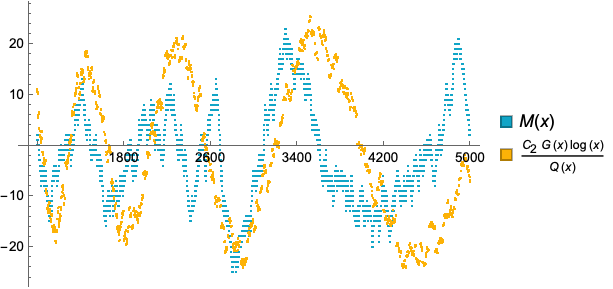
\includegraphics[width=\textwidth]{images/Figure3-CompBetweenMxAndGInvx-GInvFunctionSequenceCalculations.png}}
\captionsetup{justification=centering}
\caption{}
\end{subfigure}

\smallskip

\begin{subfigure}[t!]{\PlotFigureHorizontalScalingFactor\textwidth}
\fbox{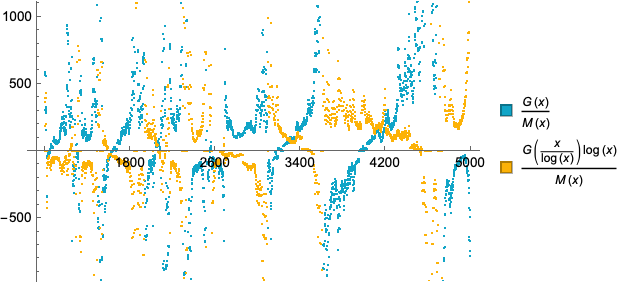
\includegraphics[width=\textwidth]{images/Figure6-RatiosOfGInvToMxAndScaledVersions-GInvFunctionSequenceCalculations.png}}
\captionsetup{justification=centering}
\caption{}
\end{subfigure}

\captionsetup{justification=centering}
\caption{} 
\label{figure_MxAndNewAuxPartialSums_Comparison_Intro_v2_v1} 

\end{figure} 

\begin{figure}[ht!]

\captionsetup{singlelinecheck=off}
\centering

\begin{subfigure}[t!]{\PlotFigureHorizontalScalingFactor\textwidth}
\fbox{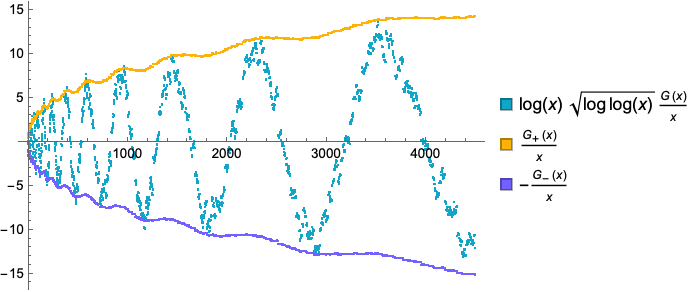
\includegraphics[width=\textwidth]{images/Figure4-ComponentsOfGInvx-GInvFunctionSequenceCalculations.png}}
\captionsetup{justification=centering}
\caption{}
\end{subfigure}

\smallskip

\begin{subfigure}[t!]{\PlotFigureHorizontalScalingFactor\textwidth}
\fbox{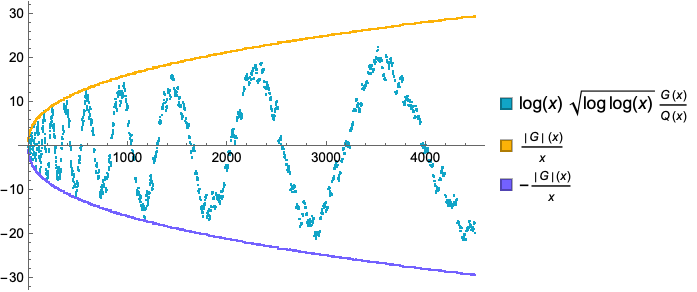
\includegraphics[width=\textwidth]{images/Figure5-ScaledGInvWithBddEnvelopes-GInvFunctionSequenceCalculations.png}}
\captionsetup{justification=centering}
\caption{}
\end{subfigure}

\captionsetup{justification=centering}
\caption{}
\label{figure_MxAndNewAuxPartialSums_Comparison_Intro_v2_v2} 

\end{figure} 

\subsection{Proofs of the new formulas} 
\label{subSection_KeyApplications_NewExactFormulasForMx} 

\begin{proof}[Proof of 
              \eqref{prop_Mx_SBP_IntegralFormula_PartA} and \eqref{prop_Mx_SBP_IntegralFormula_PartB} of 
              Theorem \hlocalref{prop_Mx_SBP_IntegralFormula}] 
By applying Theorem \hlocalref{theorem_SummatoryFuncsOfDirCvls} to 
equation \eqref{eqn_AntiqueDivisorSumIdent} we have that 
\begin{align} 
\notag
M(x) & = \sum_{k=1}^{x} \left(\pi\left(\Floor{x}{k}\right)+1\right) g(k) \\ 
\notag 
     & = G(x) + \sum_{k=1}^{\frac{x}{2}} \pi\left(\Floor{x}{k}\right) g(k) \\ 
\notag 
     & = G(x) + G\left(\Floor{x}{2}\right) + 
     \sum_{k=1}^{\frac{x}{2}-1} \left( 
     \pi\left(\Floor{x}{k}\right) - \pi\left(\Floor{x}{k+1}\right) 
	\right) G(k).
\end{align} 
The upper bound on the sum is truncated to $k \in \left[1, \frac{x}{2}\right]$ in the second equation 
above because $\pi(1) = 0$. 
The third formula above follows directly by summation by parts. 
\end{proof} 
\begin{proof}[Proof of \eqref{eqn_RmkInitialConnectionOfMxToGInvx_ProvedByInversion_v1} of 
	      Theorem \hlocalref{prop_Mx_SBP_IntegralFormula}]
Lemma \hlocalref{lemma_AnExactFormulaFor_gInvByMobiusInv_v1} shows that 
\[
G(x) = \sum_{d \leq x} \lambda(d) C_{\Omega}(d) M\left(\Floor{x}{d}\right). 
\]
The identity in \eqref{eqn_AntiqueDivisorSumIdent} implies 
$$\lambda(d) C_{\Omega}(d) = (g \ast 1)(d) = (\chi_{\mathbb{P}} + \varepsilon)^{-1}(d).$$ 
We recover the stated result from the classical inversion of summatory functions in 
equation \eqref{eqn_ApostolStmt_ClassicSummatoryFuncInvThm_v1}. 
\end{proof}

\subsection{Discrete plots and numerical experiments}

The plots shown in the figures in this section compare 
the values of $M(x)$ and $G(x)$ with scaled forms of related auxiliary partial sums: 
\begin{itemize}

\item In Figure \hlocalref{figure_MxAndNewAuxPartialSums_Comparison_Intro_v2_v1}, 
      we plot comparisons of $M(x)$ to scaled forms of $G(x)$ for $x \leq 5000$. The 
      absolute constant $C_2 := \frac{\pi^2}{6}$ where the partial sums defined by the function 
      $Q(x) := \sum_{n \leq x} \mu^2(n)$ count the number of squarefree integers $1 \leq n \leq x$. 
      In (a) the shift to the left on the $x$-axis of the former function 
      is compared and seen to be similar in shape to the magnitude of $M(x)$ on this initial subinterval. 
      It is unknown whether the similar shape and magnitude of these two functions persists for 
      much larger $x$. 
      In (b) we have observed unusual reflections and symmetry between the two ratios plotted in the 
      figure. We have numerically modified the plot values to shift the denominators of 
      $M(x)$ by one at each $x \leq 5000$ for which $M(x) = 0$. 

\item In Figure \hlocalref{figure_MxAndNewAuxPartialSums_Comparison_Intro_v2_v2}, we compare 
      envelopes on the logarithmically scaled values of $G(x) x^{-1}$ to other variants of 
      the partial sums of $g(n)$ for $x \leq 4500$. 
      In (a) we define $G(x) := G_{+}(x) - G_{-}(x)$ where the functions 
      $G_{+}(x) \geq 0$ and $G_{-}(x) \geq 0$ for all $x \geq 1$, 
      i.e., the signed component functions $G_{\pm}(x)$ 
      denote the unsigned contributions of only those summands 
      $|g(n)|$ over $n \leq x$ where $\lambda(n) = \pm 1$, respectively. 
      The summatory function $Q(x) \sim \frac{6x}{\pi^2}$ 
      in (b) has the same definition as in 
      Figure \hlocalref{figure_MxAndNewAuxPartialSums_Comparison_Intro_v2_v1} above. 
      The second plot suggests that for large $x$ 
      \[
      |G(x)| \ll \frac{|G|(x)}{(\log x) \sqrt{\log\log x}} = 
           \frac{1}{(\log x) \sqrt{\log\log x}} \times \sum_{n \leq x} |g(n)|.
      \]

\end{itemize}

\subsection{Local cancellation in 
	    the formulas involving the partial sums of $g(n)$} 
\label{subSection_LocalCancellationOfGInvx} 

\begin{definition}
Let $p_n$ denote the $n^{th}$ prime for $n \geq 1$ 
\cite[\seqnum{A000040}]{OEIS}. 
The set of primorial integers is defined by  
\cite[\seqnum{A002110}]{OEIS} 
\[
\left\{n\#\right\}_{n \geq 1} = \left\{\prod_{k=1}^{n} p_k\right\}_{n \geq 1}. 
\]
\end{definition}

\begin{prop}
\label{theorem_PrimorialSeqGInvCalcs_v1} 
As $m \rightarrow \infty$, each of the following holds: 
\begin{align} 
\tag{A} 
-G((4m+1)\#) & \asymp (4m+1)!, \\ 
\tag{B} 
G\left(\frac{(4m+1)\#}{p_k}\right) & \asymp (4m)!, 
     \mathtext{ for any } 1 \leq k \leq 4m+1. 
\end{align} 
\end{prop}
\begin{proof} 
We have by \eqref{eqn_PropB_lemma_gInv_MxExample} 
that for all squarefree integers $n \geq 1$ 
\begin{align*} 
|g(n)| & = \sum_{j=0}^{\omega(n)} \binom{\omega(n)}{j} \times j! 
     = (\omega(n))! \times \sum_{j=0}^{\omega(n)} \frac{1}{j!} \\ 
     & = (\omega(n))! \times \left(e + O\left(\frac{1}{(\omega(n)+1)!}\right)\right). 
\end{align*} 
Let $m$ be a large positive integer. 
We obtain main terms of the form 
\begin{align} 
\label{eqn_proof_tag_GinvxLocalCancellation_v1} 
\sum_{\substack{n \leq (4m+1)\# \\ \omega(n)=\Omega(n)}} \lambda(n) |g(n)| 
     & = \sum_{0 \leq k \leq 4m+1} \binom{4m+1}{k} (-1)^{k} k! \times 
     \left(e + O\left(\frac{1}{(k+1)!}\right)\right) \\ 
\notag 
     & = -(4m+1)! + O\left(\frac{1}{4m+1}\right). 
\end{align} 
The formula for $C_{\Omega}(n)$ stated in 
\eqref{eqn_proof_tag_hInvn_ExactNestedSumFormula_CombInterpetIdent_v3} 
implies the result in (A). 
This happens because the contributions from the summands of the inner 
summation on the right-hand-side of 
\eqref{eqn_proof_tag_GinvxLocalCancellation_v1} 
off of the squarefree integers 
are at most a bounded multiple of $(-1)^k \times k!$ when $\Omega(n) = k$. 

We can similarly show that for any $1 \leq k \leq 4m+1$ 
\begin{align*}
G\left(\frac{(4m+1)\#}{p_k}\right) & \asymp \sum_{0 \leq k \leq 4m} \binom{4m}{k} (-1)^{k} k! 
     \times \left(e + O\left(\frac{1}{(k+1)!}\right)\right) = (4m)! + O\left(\frac{1}{4m+1}\right). 
     \qedhere 
\end{align*}
\end{proof}

\begin{remark}
\label{remark_LocalCancellationWithGxAlongThePrimorialsUnderTheRH} 
The Riemann hypothesis (RH) is equivalent to showing that 
\begin{equation} 
\label{eqn_MertensMx_RHEquivProblem_Stmt_intro} 
M(x) = O\left(x^{\frac{1}{2}+\varepsilon}\right), \mathtext{ for all } 0 < \varepsilon < \frac{1}{2}.
\end{equation}
We expect that there is usually (almost always) 
a large amount cancellation between the successive 
values of the summatory function in 
\eqref{eqn_RmkInitialConnectionOfMxToGInvx_ProvedByInversion_v1}. 
Proposition \hlocalref{theorem_PrimorialSeqGInvCalcs_v1} 
demonstrates the phenomenon well along the infinite 
subsequence of the primorials $\{(4m+1)\#\}_{m \geq 1}$. 
If the RH is true, the sums of the leading constants with opposing signs 
on the asymptotic bounds for the functions from the last proposition 
are necessarily required to match. 
In particular, we have that 
\cite{DUSART-1999,DUSART-2010} 
\[
n\# \sim e^{\vartheta(p_n)} \asymp n^n (\log n)^n e^{-n(1+o(1))}, 
     \mathtext{ as } n \rightarrow \infty. 
\]
The observation on the necessary cancellation in 
\eqref{eqn_RmkInitialConnectionOfMxToGInvx_ProvedByInversion_v1}
follows from the fact that if we obtain a contrary result, 
then for some fixed $\delta_0 > 0$
\[
\frac{M((4m+1)\#)}{\sqrt{(4m+1)\#}} \gg \left[(4m+1)\#\right]^{\delta_0}, 
     \mathtext{ as } m \rightarrow \infty. 
\]
If the last equation holds, then we would find a contradiction to 
equation \eqref{eqn_MertensMx_RHEquivProblem_Stmt_intro}. 
Assuming the RH, we can state a stronger bound for the 
Mertens function along this subsequence by considering the 
error terms given in the proof of 
Proposition \hlocalref{theorem_PrimorialSeqGInvCalcs_v1}. 
\end{remark}

\section{Conclusions}

\subsection{Summary}

We have identified a sequence, 
$\{g(n)\}_{n \geq 1}$, that is the Dirichlet inverse of the 
shifted strongly additive function $\omega(n)$. 
There is a natural 
combinatorial interpretation to the repetition of distinct values 
of $|g(n)|$ in terms of the configuration of the 
exponents in the prime factorization of any $n \geq 2$. 
The sign of $g(n)$ is given by $\lambda(n)$ for all $n \geq 1$. 
This leads to a new relations between the 
summatory function $G(x)$ to $M(x)$ and $L(x)$. 
We have also formalized a new perspective from which we might express 
our intuition about features of the distribution of $G(x)$ 
via the properties of its $\lambda(n)$-sign-weighted summands.
The new results proved within this article 
are significant in providing a new window through which we can view $M(x)$ 
in terms of the unsigned sequences and their partial sums. 

\subsection{Discussion of the new results}

Probabilistic models of the M\"obius function lead us to consider the behavior of $M(x)$ 
as a sum of independent and identically distributed (i.i.d.) random variables. 
Suppose that $\{X_n\}_{n \geq 1}$ is a sequence of i.i.d. 
$\{-1,0,1\}$-valued random variables 
such that for all $n \geq 1$ 
$$\mathbb{P}[X_n = -1] = \mathbb{P}[X_n = +1] = \frac{3}{\pi^2}, 
  \mathtext{ and } \mathbb{P}[X_n = 0] = 1 - \frac{6}{\pi^2},$$ 
i.e., so that the sequence provides a randomized model of the values of $\mu(n)$ on the average. 
We may then approximate the partial sums as 
$M(x) \cong S_x$ where $S_x := \sum_{n \leq x} X_n$ for all $x \geq 1$. 
This viewpoint models predictions of certain limiting asymptotic behavior of the 
Mertens function including \cite[\S TODO]{TODO-PROB-BOOK}
\[
\mathbb{E}\left[S_x\right] = 0, 
     \operatorname{Var}\left[S_x\right] = \frac{6x}{\pi^2}, 
     \mathtext{ and } 
     \limsup_{x \rightarrow \infty} \frac{\left\lvert S_x\right\rvert}{\sqrt{x \log\log x}} = 
     \frac{2\sqrt{3}}{\pi} \mathtext{ (almost surely).} 
\]
The Mertens function is related to the partial sums in 
\eqref{eqn_LxSummatoryFuncDef_v1} 
via the relation \cite{HUMPHRIES-JNT-2013,LEHMAN-1960} 
\begin{equation}
\label{eqn_MxInTermsOfLx_v1} 
M(x) = \sum_{d \leq \sqrt{x}} \mu(d) L\left(\Floor{x}{d^2}\right), \mathtext{ for } x \geq 1.
\end{equation}
The relation in \eqref{eqn_MxInTermsOfLx_v1} 
gives an exact expression for $M(x)$ with summands involving $L(x)$ that are oscillatory. 
In contrast, the exact expansions for the Mertens function given in 
Theorem \hlocalref{prop_Mx_SBP_IntegralFormula} 
express $M(x)$ as finite sums over $\lambda(n)$ with weighted coefficients that are unsigned. 
The property of the symmetry of the distinct values of $|g(n)|$ with respect to the 
prime factorizations of $n \geq 2$ in \eqref{eqn_FactSymmPropertyOfgn_v1} 
suggests that the unsigned weights on $\lambda(n)$ in 
the new formulas from the theorem yield new insights compared to 
equation \eqref{eqn_MxInTermsOfLx_v1} as confirmed by 
Theorem \hlocalref{cor_CLT_VII}. 

Stating tight bounds on the distribution of 
$L(x)$ is a problem that is equally as difficult 
as understanding the growth of $M(x)$
along infinite subsequences (\cf \cite{MR2877066,MR3779960,TAO-LOGAVGD-CHOWLA}). 
Indeed, $\lambda(n) = \mu(n)$ for all squarefree $n \geq 1$ so that 
$\lambda(n)$ agrees with $\mu(n)$ at most large $n$. 
We infer that $\lambda(n)$ must inherit the pseudo-randomized quirks 
of $\mu(n)$ predicted by Sarnak's conjecture. 
On the other hand, the formulas in 
Theorem \hlocalref{prop_Mx_SBP_IntegralFormula} are more desirable to explore than 
other classical formulae for $M(x)$ for the following reasons:
\begin{itemize}
\item Breakthrough work in recent years due to 
	Matom\"aki, Radziwi{\l\l} and Soundararajan to 
	bound multiplicative functions 
	in short intervals has 
	proven fruitful when applied to $\lambda(n)$ 
	\cite{SOUND-LLAMBDA-SHORT-INTS,MATRADZE-MULTFUNCS-SHORT-INTS}. 
	The analogs of results of this type corresponding 
	to the M\"obius function are not clearly attained; 
\item The squarefree $n \geq 1$ on which $\lambda(n)$ and $\mu(n)$ must identically agree 
	are in some senses easier integer cases to handle 
	insomuch as we can prove very regular properties 
	that govern the distributions of the distinct values of 
	$\omega(n)$, $\Omega(n)$ and their difference over $n \leq x$ as $x \rightarrow \infty$ 
	\citep[\cf \S 2.4; \S 7.4]{MV}; 
\item The function $\lambda(n)$ is completely 
	multiplicative. Hence, the function $\lambda(n)$ may be 
	a nicer cousin to the multiplicative $\mu(n)$ on the 
	integers $n \geq 4$ for which $\mu(n) = 0$. 
\end{itemize}

\subsection{Future work} 
\label{remark_ConjPropApps_SumsOfGx_v1} 

One obvious application of 
Theorem \hlocalref{cor_CLT_VII} 
is to apply the limiting distribution of $|g(n)|$ to find 
new asymptotic bounds for the $\lambda(n)$-signed summands of the 
partial sums of $g(n)$. 
The large order growth of the average order of $|g(n)|$ is problematic in 
predicting the likelihood (on average) that 
$\left\lvert \sum_{n \leq x} g(n) \right\rvert \leq T$ for any fixed $T > 0$. 
We expect enormous cancellation almost everywhere 
in the summatory function terms in 
\eqref{eqn_RmkInitialConnectionOfMxToGInvx_ProvedByInversion_v1} of 
Theorem \hlocalref{prop_Mx_SBP_IntegralFormula}. 
A possible extension of this work is to find new ways to 
exploit the cancellation in this formula to extract 
hidden information about the frequency of the sign changes of $\lambda(n)$ 
on bounded subintervals of $[1, x]$ based on the large expected spread of the functions in 
Theorem \hlocalref{cor_CLT_VII} as $x \rightarrow \infty$ 
(\cf Section \hlocalref{subSection_RemarksOnAvgOrderFor_COmegan_directly_SelbergDelangeMethod}). 

\renewcommand{\refname}{References} 
\addcontentsline{toc}{section}{References}
\bibliography{glossaries-bibtex/thesis-references}{}
\bibliographystyle{plain}

\begin{thebibliography}{10}

\bibitem{APOSTOLANUMT}
T.~M. Apostol.
\newblock {\em Introduction to Analytic Number Theory}.
\newblock Springer--Verlag, 1976.

\bibitem{ANT-BATEMAN-DIAMOND}
P.~T. Bateman and H.~G. Diamond.
\newblock {\em Analytic Number Theory}.
\newblock World Scientific Publishing, 2004.

\bibitem{BILLINGSLY-CLT-PRIMEDIVFUNC}
P.~Billingsley.
\newblock On the central limit theorem for the prime divisor function.
\newblock {\em Amer. Math. Monthly}, 76(2):132--139, 1969.

\bibitem{BILLINGSLY-PROB-AND-MEASURE-BOOK}
P.~Billingsley.
\newblock {\em Probability and measure}.
\newblock Wiley, third edition, 1994.

\bibitem{DUSART-1999}
P.~Dusart.
\newblock The $k^{th}$ prime is greater than $k(\log k +\log\log k-1)$ for $k
  \geq 2$.
\newblock {\em Math. Comp.}, 68(225):411--415, 1999.

\bibitem{DUSART-2010}
P.~Dusart.
\newblock Estimates of some functions over primes without {R}.{H}., 2010.

\bibitem{ELLIOTT-V1}
P.~D. T.~A. Elliott.
\newblock {\em Probabilistic Number Theory {I}: Mean-Value Theorems}.
\newblock Springer New York, 1979.

\bibitem{ERDOS-KAC-REF}
P.~Erd{\H{o}}s and M.~Kac.
\newblock The {G}aussian errors in the theory of additive arithmetic functions.
\newblock {\em American Journal of Mathematics}, 62(1):738--742, 1940.

\bibitem{MR3779960}
N.~Frantzikinakis and B.~Host.
\newblock The logarithmic {S}arnak conjecture for ergodic weights.
\newblock {\em Ann. of Math. (2)}, 187(3):869--931, 2018.

\bibitem{FROBERG-1968}
C.~E. Fr{\"{o}}berg.
\newblock On the prime zeta function.
\newblock {\em BIT Numerical Mathematics}, 8:87--202, 1968.

\bibitem{MR2877066}
B.~Green and T.~Tao.
\newblock The {M}\"{o}bius function is strongly orthogonal to nilsequences.
\newblock {\em Ann. of Math. (2)}, 175(2):541--566, 2012.

\bibitem{HARDYWRIGHT}
G.~H. Hardy and E.~M. Wright, editors.
\newblock {\em An Introduction to the Theory of Numbers}.
\newblock Oxford University Press, 2008 (Sixth Edition).

\bibitem{HUMPHRIES-JNT-2013}
P.~Humphries.
\newblock The distribution of weighted sums of the {L}iouville function and
  {P}\'{o}lya's conjecture.
\newblock {\em J. Number Theory}, 133:545--582, 2013.

\bibitem{LEHMAN-1960}
R.~S. Lehman.
\newblock On {L}iouville's function.
\newblock {\em Math. Comput.}, 14:311--320, 1960.

\bibitem{MATRADZE-MULTFUNCS-SHORT-INTS}
K.~Matom{\"{a}}ki and M.~Radziwi{\l\l}.
\newblock Multiplicative functions in short intervals.
\newblock {\em Ann. of Math.}, 183:1015--1056, 2016.

\bibitem{MV}
H.~L. Montgomery and R.~C. Vaughan.
\newblock {\em Multiplicative Number Theory: I, Classical Theory}.
\newblock Cambridge, 2006.

\bibitem{NEMES2015C}
G.~Nemes.
\newblock The resurgence properties of the incomplete gamma function {II}.
\newblock {\em Stud. Appl. Math.}, 135(1):86--116, 2015.

\bibitem{NEMES2016}
G.~Nemes.
\newblock The resurgence properties of the incomplete gamma function {I}.
\newblock {\em Anal. Appl. (Singap.)}, 14(5):631--677, 2016.

\bibitem{NEMES2019}
G.~Nemes and A.~B.~Olde Daalhuis.
\newblock Asymptotic expansions for the incomplete gamma function in the
  transition regions.
\newblock {\em Math. Comp.}, 88(318):1805--1827, 2019.

\bibitem{NISTHB}
F.~W.~J. Olver, D.~W. Lozier, R.~F. Boisvert, and C.~W. Clark, editors.
\newblock {\em {NIST} Handbook of Mathematical Functions}.
\newblock Cambridge University Press, 2010.

\bibitem{LOG-COMB-STRUCTS-BOOK}
A.~D.~Barbour R.~Arratia and Simon Tavar{\'{e}}.
\newblock {\em Logarithmic Combinatorial Structures: A Probabilistic Approach}.
\newblock Preprint draft, 2002.

\bibitem{OEIS}
N.~J.~A. Sloane.
\newblock The {O}nline {E}ncyclopedia of {I}nteger {S}equences, 2021.
\newblock \url{http://oeis.org}.

\bibitem{SOUND-LLAMBDA-SHORT-INTS}
K.~Soundararajan.
\newblock The {L}iouville function in short intervals (after {M}atom{\"{a}}ki
  and {R}adziwi{\l}{\l}).
\newblock {\em arXiv:1606.08021}, 2016.

\bibitem{TAO-LOGAVGD-CHOWLA}
T.~Tao.
\newblock The logarithmically averaged {C}howla and {E}lliott conjectures for
  two-point correlations.
\newblock {\em Forum of Mathematics}, 4:e8, 2016.

\bibitem{TENENBAUM-PROBNUMT-METHODS}
G.~Tenenbaum.
\newblock {\em Introduction to Analytic and Probabilistic Number Theory}.
\newblock American Mathematical Society, 2015.

\end{thebibliography}

\appendix
\cftaddtitleline{toc}{section}{Appendices on supplementary material}{}
\setcounter{section}{0} 
\renewcommand{\thesection}{\Alph{section}} 

\smallskip\hrule\hrule\hrule\hrule\hrule\hrule\smallskip
%{\huge{\textbf{Appendices on supplementary material}}} 
%\medskip\hrule\hrule\hrule\hrule\hrule\hrule\smallskip

%\section{Glossary of notation and conventions}
%\label{Section_NotationAndConventions}
%
%\renewcommand*{\glsclearpage}{}
%\renewcommand{\glossarysection}[2][]{}
%\vspace*{-0.56cm}
%\printglossary[type={symbols},
%               style={glossstyleSymbol},
%               nogroupskip=true]

\section{The distributions of $\omega(n)$ and $\Omega(n)$ (TODO)} 
\label{subSection_TheKnownDistsOfThePrimeOmegaFunctions_IntroResults_v1} 

As $n \rightarrow \infty$, we have that 
$$\frac{1}{n} \times \sum_{k \leq n} \omega(k) = \log\log n + B_1 + o(1),$$ 
and 
$$\frac{1}{n} \times \sum_{k \leq n} \Omega(k) = \log\log n + B_2 + o(1),$$ 
where $B_1 \approx 0.261497$ and $B_2 \approx 1.03465$ are 
absolute constants \cite[\S 22.10]{HARDYWRIGHT}. 
The next theorems reproduced from \cite[\S 7.4]{MV} bound the frequency of the 
number of times $\Omega(n)$ $n \leq x$ 
diverges substantially from its average order at integers $n \leq x$ 
when $x$ is large 
(\cf \cite{ERDOS-KAC-REF,BILLINGSLY-CLT-PRIMEDIVFUNC}). 

\begin{theorem}[Rankin's method] 
\label{theorem_MV_Thm7.20-init_stmt} 
For $x \geq 2$ and $r > 0$, let 
\begin{align*} 
A(x, r) & := \#\left\{n \leq x: \Omega(n) \leq r \log\log x\right\}, \\ 
B(x, r) & := \#\left\{n \leq x: \Omega(n) \geq r \log\log x\right\}. 
\end{align*} 
If $0 < r \leq 1$, then 
\[
A(x, r) \ll\phantom{_R} x (\log x)^{r-1 - r\log r}, \mathtext{ as } x \rightarrow \infty. 
\]
If $1 \leq r \leq R < 2$, then 
\[
B(x, r) \ll_R x (\log x)^{r-1-r \log r}, \mathtext{ as } x \rightarrow \infty. 
\]
\end{theorem} 

\begin{theorem}
\label{theorem_HatPi_ExtInTermsOfGz} 
For integers $k \geq 1$ and $x \geq 2$ 
$$\widehat{\pi}_k(x) := \#\{1 \leq n \leq x: \Omega(n)=k\}.$$ 
For $0 < R < 2$, uniformly for $1 \leq k \leq R \log\log x$ 
\begin{equation}
\label{eqn_PiHatkx_UniformAsymptoticsStmt_from_MV_v1}
\widehat{\pi}_k(x) = \frac{x}{\log x} \times \mathcal{G}\left(\frac{k-1}{\log\log x}\right) 
     \frac{(\log\log x)^{k-1}}{(k-1)!} \left(1 + O_R\left(\frac{k}{(\log\log x)^2}\right)\right), 
     \mathtext{ as } x \rightarrow \infty. 
\end{equation}
For $0 \leq |z| < R$, the leading factor in 
equation \eqref{eqn_PiHatkx_UniformAsymptoticsStmt_from_MV_v1} 
is defined in terms of the function 
\[
\mathcal{G}(z) := \frac{1}{\Gamma(1+z)} \times 
	\prod_p \left(1-\frac{z}{p}\right)^{-1} \left(1-\frac{1}{p}\right)^z. 
\]
\end{theorem} 

We can extend the proofs in \cite[\S 7]{MV} to obtain 
results on the distribution of $\omega(n)$. 

\begin{remark} 
\label{remark_MV_Pikx_FuncResultsAnnotated_v1} 
For integers $k  \geq 1$ and $x \geq 2$, we define 
\[
\pi_k(x) := \#\{2 \leq n \leq x: \omega(n)=k\}.
\]
For fixed $0 < R < 2$, as $x \rightarrow \infty$ we have 
uniformly for $1 \leq k \leq R\log\log x$ that 
\begin{equation}
\label{eqn_Pikx_UniformAsymptoticsStmt_from_MV_v2} 
\pi_k(x) = \frac{x}{\log x} \times 
     \widetilde{\mathcal{G}}\left(\frac{k-1}{\log\log x}\right) 
     \frac{(\log\log x)^{k-1}}{(k-1)!} \left( 
     1 + O_R\left(\frac{k}{(\log\log x)^2}\right) 
     \right). 
\end{equation}
The leading factor in 
equation \eqref{eqn_Pikx_UniformAsymptoticsStmt_from_MV_v2} 
is defined in terms of the function 
\[
\widetilde{\mathcal{G}}(z) := \frac{1}{\Gamma(1+z)} \times 
	\prod_p \left(1 + \frac{z}{p-1}\right) \left(1 - \frac{1}{p}\right)^{z}, 
	\mathtext{ for } |z| \leq R < 2. 
\]
\end{remark} 

\section{The incomplete gamma function (TODO)} 
\label{subSection_OtherFactsAndResults} 

We cite correspondence online with Gerg\H{o} Nemes 
from the Alfr\'{e}d R\'{e}nyi Institute of Mathematics and thank him for his 
notes on asymptotics for the sums in this section. 
These proofs are adapted below based on his work in 
\cite{NEMES2015C,NEMES2016,NEMES2019}. 

\begin{definition}
The (upper) incomplete gamma function is defined by \cite[\S 8.4]{NISTHB} 
\[
\Gamma(a, z) = \int_{z}^{\infty} t^{a-1} e^{-t} dt, \mathtext{ for } 
	a \in \mathbb{R} \mathtext{ and } |\arg z| < \pi.  
\]
\end{definition}

The function $\Gamma(a, z)$ can be continued to an analytic function of $z$ on the 
universal covering of $\mathbb{C} \mathbin{\backslash} \{0\}$. 
For $a \in \mathbb{Z}^{+}$, the function $\Gamma(a, z)$ is an entire function of $z$. 

\begin{facts} 
\label{facts_ExpIntIncGammaFuncs} 
\begin{subequations}
The following properties hold \cite[\S 8.4; \S 8.11(i)]{NISTHB}: 
\begin{align} 
\label{eqn_IncompleteGamma_PropA} 
     \Gamma(a, z) & = (a-1)! e^{-z} \times \sum_{k=0}^{a-1} \frac{z^k}{k!}, \mathtext{ for } 
     a \in \mathbb{Z}^{+} \mathtext{ and } z \in \mathbb{C}, \\ 
\label{eqn_IncompleteGamma_PropB} 
\Gamma(a, z) & \sim z^{a-1} e^{-z}, \mathtext{ for fixed } a \in \mathbb{R} 
     \mathtext{ and } z > 0 \mathtext{ as } z \rightarrow \infty. 
\end{align}
For $z > 0$, as $z \rightarrow \infty$ we have that \cite{NEMES2015C} 
\begin{equation} 
\label{eqn_IncompleteGamma_PropC}
\Gamma(z, z) = \sqrt{\frac{\pi}{2}} z^{z-\frac{1}{2}} e^{-z}\left(
	1 + O\left(\frac{1}{\sqrt{z}}\right)\right). 
\end{equation} 
For fixed, finite real $|\rho| > 0$, we define the sequence 
$\{b_n(\rho)\}_{n \geq 0}$ by the following recurrence relation: 
\[
b_n(\rho) = \rho \cdot (1-\rho) b_{n-1}^{\prime}(\rho) + 
	\rho \cdot (2n-1) b_{n-1}(\rho) + \delta_{n,0}. 
\]
If $z,a \rightarrow \infty$ with $z = \rho a$ for some $\rho > 1$ such that 
$(\rho - 1)^{-1} = o\left(\sqrt{|a|}\right)$, then \cite{NEMES2015C}
\begin{equation}
\label{eqn_IncompleteGamma_PropD}
\Gamma(a, z) \sim z^a e^{-z} \times \sum_{n \geq 0} \frac{(-a)^n b_n(\rho)}{(z-a)^{2n+1}}. 
\end{equation} 
\end{subequations}
\end{facts} 

\begin{prop}
\label{prop_IncGammaLambdaTypeBounds_v1}
\begin{subequations}
Let $a,z,\rho$ be positive real parameters such that $z \sim \rho a$. 
If $\rho \in (0, 1)$, then as $z \rightarrow \infty$ 
\begin{equation}
\Gamma(a, z) = \Gamma(a) + O_{\rho}\left(z^{a-1} e^{-z}\right). 
\end{equation}
If $\rho > 1$, then as 
$z \rightarrow \infty$ 
\begin{equation}
\Gamma(a, z) = \frac{z^{a-1} e^{-z}}{1-\rho^{-1}} + O_{\rho}\left(z^{a-2} e^{-z}\right). 
\end{equation}
If $\rho > W(1)$, then as $z \rightarrow \infty$ 
\begin{equation}
\Gamma(a, z e^{\pm\pi\imath}) = -e^{\pm \pi\imath a} \frac{z^{a-1} e^{z}}{1 + \rho^{-1}} + 
     O_{\rho}\left(z^{a-2} e^{z}\right). 
\end{equation}
\end{subequations}
\end{prop}

\begin{remark}
The first two estimates in the proposition 
are only useful when $\rho$ is bounded away from the transition point at one. 
We cannot write the last expansion above 
as $\Gamma(a, -z)$ directly unless $a \in \mathbb{Z}^{+}$ 
as the incomplete gamma function 
has a branch point at the origin with respect to its second variable. 
This function becomes a single-valued 
analytic function of its second input by continuation 
on the universal covering of $\mathbb{C} \mathbin{\backslash} \{0\}$. 
\end{remark}

\begin{proof}[Proof of Proposition \hlocalref{prop_IncGammaLambdaTypeBounds_v1}] 
The first asymptotic estimate follows directly from the following 
asymptotic series expansion that holds as $z \rightarrow \infty$ 
\cite[Eq.\ (2.1)]{NEMES2019}: 
\[
\Gamma(a, z) \sim \Gamma(a) + z^a e^{-z} \times \sum_{k \geq 0} 
     \frac{(-a)^k b_k(\rho)}{(z-a)^{2k+1}}. 
\]
Using the notation from \eqref{eqn_IncompleteGamma_PropD} and \cite{NEMES2016} 
\[
\Gamma(a, z) = \frac{z^{a-1} e^{-z}}{1-\rho^{-1}} + z^{a} e^{-z} R_1(a, \rho). 
\]
From the bounds in \cite[\S 3.1]{NEMES2016}, we have 
\[
\left\lvert z^{a} e^{-z} R_1(a, \rho) \right\rvert \leq 
     z^a e^{-z} \times \frac{a \cdot b_1(\rho)}{(z-a)^{3}} = 
     \frac{z^{a-2} e^{-z}}{(1-\rho^{-1})^{3}}
\]
The main and error terms in the previous equation can also be 
seen by applying the asymptotic series in 
\eqref{eqn_IncompleteGamma_PropD} directly. 

The proof of the third equation above follows from the asymptotics 
\cite[Eq.\ (1.1)]{NEMES2015C}
\[
\Gamma(-a, z) \sim z^{-a} e^{-z} \times \sum_{n \geq 0} \frac{a^n b_n(-\rho)}{(z+a)^{2n+1}}, 
\]
by setting $(a, z) \mapsto \left(a e^{\pm \pi\imath}, z e^{\pm \pi\imath}\right)$ so that 
$\rho = \frac{z}{a} > W(1) \approx 0.56714$. 
The restriction on the range of $\rho$ over which the third formula holds is made to ensure that 
the formula from the reference is valid at negative real $a$. 
\end{proof}

\begin{lemma}
\label{lemma_ConvenientIncGammaFuncTypePartialSumAsymptotics_v2}
As $x \rightarrow \infty$  
\begin{align*}
\frac{x}{\log x} \times \left\lvert \sum_{1 \leq k \leq \log\log x} 
     \frac{(-1)^k (\log\log x)^{k-1}}{(k-1)!} \right\rvert 
     & = \frac{x}{2\sqrt{2\pi \log\log x}} 
     \left(1 + O\left(\frac{1}{\log\log x}\right)\right). 
\end{align*}
\end{lemma}
\begin{proof}
We have for $n \geq 1$ and any $t > 0$ by 
\eqref{eqn_IncompleteGamma_PropA} that 
\[
\sum_{1 \leq k \leq n} \frac{(-1)^k t^{k-1}}{(k-1)!} = -e^{-t} \times 
     \frac{\Gamma(n, -t)}{(n-1)!}. 
\]
Suppose that $t = n + \xi$ with $\xi = O(1)$. 
By the third formula 
in Proposition \hlocalref{prop_IncGammaLambdaTypeBounds_v1} 
with the parameters $(a, z, \lambda) \mapsto \left(n, t, 1 + \frac{\xi}{n}\right)$, 
we deduce that as $n,t \rightarrow \infty$. 
\begin{equation*}
\Gamma(n, -t) = (-1)^{n+1} \times \frac{t^n e^{t}}{t+n} + 
     O\left(\frac{n t^n e^{t}}{(t+n)^3}\right) = 
     \frac{(-1)^{n+1} t^n e^t}{2n} + O\left(\frac{t^{n-1} e^t}{n}\right). 
\end{equation*}
Accordingly, we see that 
\[
\sum_{1 \leq k \leq n} \frac{(-1)^k t^{k-1}}{(k-1)!} = 
      \frac{(-1)^{n} t^n}{2n!} + O\left(\frac{t^{n-1}}{n!}\right). 
\]
By the form of Stirling's formula in \cite[\cf Eq.\ (5.11.8)]{NISTHB}, we have 
\[
n! = \Gamma(1 + t - \xi) = \sqrt{2\pi} t^{t-\xi+\frac{1}{2}} e^{-t} \left(1 + O\left(t^{-1}\right)\right) = 
     \sqrt{2\pi} t^{n+\frac{1}{2}} e^{-t} \left(1 + O\left(t^{-1}\right)\right). 
\]
Hence, as $n \rightarrow \infty$ with $t := n + \xi$ and $\xi = O(1)$, we obtain that 
\[
\sum_{k=1}^{n} \frac{(-1)^k t^{k-1}}{(k-1)!} = \frac{(-1)^n e^t}{2 \sqrt{2\pi t}} + 
     O\left(e^t t^{-\frac{3}{2}}\right). 
\]
The conclusion follows by taking $n := \floor{\log\log x}$ and $t := \log\log x$. 
\end{proof}

An adaptation of the proof of 
Lemma \hlocalref{lemma_ConvenientIncGammaFuncTypePartialSumAsymptotics_v2} 
shows that for any $a \in \left(1, W(1)^{-1}\right) \subset (1, 1.76321)$ 
\begin{align*}
\frac{x}{\log x} \times \left\lvert \sum_{k=1}^{a \log\log x} 
     \frac{(-1)^{k} (\log\log x)^{k-1}}{(k-1)!} 
     \right\rvert = 
     \frac{\sqrt{a} x}{\sqrt{2\pi}(a+1) a^{\{a\log\log x\}}} 
     \times \frac{(\log x)^{a-1-a\log a}}{\sqrt{\log\log x}} 
     \left(1 + O\left(\frac{1}{\log\log x}\right)\right). 
\end{align*}
The function $\{x\} = x - \floor{x} \in [0, 1)$ denotes the fractional part of 
any $x \in \mathbb{R}$.
The function $a-1-a\log a$ is negative and monotone decreasing for $a$ on 
$\left(1, W(1)^{-1}\right)$. 

\section{Inversion of partial sums of Dirichlet convolutions}
\label{Section_PrelimProofs_Config} 
\label{subSection_PrelimProofs_Config_InversionTheorem}

\begin{proof}[Proof of Theorem \hlocalref{theorem_SummatoryFuncsOfDirCvls}] 
\label{proofOf_theorem_SummatoryFuncsOfDirCvls} 
Suppose that $h,r$ are arithmetic functions such that $r(1) \neq 0$, i.e., so that 
the function $r$ is invertible with respect to the operation of Dirichlet convolution. 
The following formulas hold for all $x \geq 1$: 
\begin{align} 
\notag 
S_{r \ast h}(x) & := \sum_{n=1}^{x} \sum_{d|n} r(n) h\left(\frac{n}{d}\right) = 
     \sum_{d=1}^x r(d) \times H\left(\floor{\frac{x}{d}}\right) \\ 
\label{eqn_proof_tag_PigAsthx_ExactSummationFormula_exp_v2} 
     & \phantom{:} = 
     \sum_{i=1}^x \left(R\left(\floor{\frac{x}{i}}\right) - R\left(\floor{\frac{x}{i+1}}\right)\right) H(i). 
\end{align} 
The first formula on the right-hand-side above is well known from the references. 
The second formula is justified directly using 
summation by parts as \cite[\S 2.10(ii)]{NISTHB} 
\begin{align*} 
S_{r \ast h}(x) & = \sum_{d=1}^x h(d) \times R\left(\floor{\frac{x}{d}}\right) \\ 
     & = \sum_{i \leq x} \left(\sum_{j \leq i} h(j)\right) \times 
     \left(R\left(\floor{\frac{x}{i}}\right) - 
     R\left(\floor{\frac{x}{i+1}}\right)\right). 
\end{align*} 
For Boolean-valued conditions \texttt{cond}, we adopt Iverson's convention that 
$\Iverson{\mathtt{cond}}$ evaluates to one precisely when 
\texttt{cond} is true and to zero otherwise.
We form the invertible matrix of coefficients (denoted by $\hat{R}$ below) 
associated with the linear system that defines $H(j)$ for 
$1 \leq j \leq x$ in \eqref{eqn_proof_tag_PigAsthx_ExactSummationFormula_exp_v2} by defining
\[
R_{x,j} := R\left(\Floor{x}{j}\right) \Iverson{j \leq x}, 
\]
and 
\[
r_{x,j} := R_{x,j} - R_{x,j+1}, \mathtext{ for } 1 \leq j \leq x. 
\] 
Since $r_{x,x} = R(1) = r(1) \neq 0$ for all $x \geq 1$ and $r_{x,j} = 0$ for all $j > x$, 
the matrix we have defined in this problem is lower triangular with a non-zero 
constant on its diagonals, and so is invertible. 
If we let $\hat{R} := (R_{x,j})$, then the next matrix is 
expressed by applying an invertible shift operation as 
\[
(r_{x,j}) = \hat{R} \left(I - U^{T}\right). 
\]
The $N \times N$ square matrix $U$ 
has $(i,j)^{th}$ entries for all $1 \leq i,j \leq N$ when $N \geq x$ that are defined by 
$(U)_{i,j} = \delta_{i+1,j}$ so that 
\[
\left[\left(I - U^T\right)^{-1}\right]_{i,j} = \Iverson{j \leq i}. 
\]
We observe that 
\[
\Floor{x}{j} - \Floor{x-1}{j} = \begin{cases} 
     1, & \text{ if $j|x$; } \\ 
     0, & \text{ otherwise. } 
     \end{cases} 
\] 
The previous equation implies that 
\begin{equation} 
\label{eqn_proof_tag_FloorFuncDiffsOfSummatoryFuncs_v2} 
R\left(\floor{\frac{x}{j}}\right) - R\left(\floor{\frac{x-1}{j}}\right) = 
     \begin{cases} 
     r\left(\frac{x}{j}\right), & \text{ if $j|x$; } \\ 
     0, & \text{ otherwise. } 
     \end{cases}
\end{equation} 
We use the property in \eqref{eqn_proof_tag_FloorFuncDiffsOfSummatoryFuncs_v2} 
to shift the matrix $\hat{R}$, and then invert the result to obtain a matrix involving the 
Dirichlet inverse of $r$ as 
\begin{align*} 
\left(\left(I-U^{T}\right) \hat{R}\right)^{-1} & = 
     \left(r\left(\frac{x}{j}\right) \Iverson{j|x}\right)^{-1} = 
     \left(r^{-1}\left(\frac{x}{j}\right) \Iverson{j|x}\right). 
\end{align*} 
Our target matrix is 
$$(r_{x,j}) = \left(I-U^{T}\right) \left(r\left(\frac{x}{j}\right) \Iverson{j|x}\right) \left(I-U^{T}\right)^{-1}.$$
We can express its inverse by a similarity transformation conjugated by shift operators by 
\begin{align*} 
(r_{x,j})^{-1} & = \left(I-U^{T}\right)^{-1} \left(r^{-1}\left(\frac{x}{j}\right) 
     \Iverson{j|x}\right) \left(I-U^{T}\right) \\ 
     & = \left(\sum_{k=1}^{\floor{\frac{x}{j}}} r^{-1}(k)\right) \left(I-U^{T}\right) \\ 
     & = \left(\sum_{k=1}^{\floor{\frac{x}{j}}} r^{-1}(k) - \sum_{k=1}^{\floor{\frac{x}{j+1}}} r^{-1}(k)\right). 
\end{align*} 
The summatory function $H(x)$ is given exactly 
by a vector product with the inverse matrix from the previous equation as 
\begin{align*} 
H(x) & = \sum_{k=1}^x \left(\sum_{j=\floor{\frac{x}{k+1}}+1}^{\floor{\frac{x}{k}}} r^{-1}(j)\right) 
	\times S_{r \ast h}(k), \mathtext{ for } x \geq 1. 
\end{align*} 
We can prove a second inversion formula by adapting our argument used to prove 
\eqref{eqn_proof_tag_PigAsthx_ExactSummationFormula_exp_v2} above. 
This leads to the alternate expression for $H(x)$ given by 
\[
H(x) = \sum_{k=1}^{x} r^{-1}(k) \times S_{r \ast h}\left(\Floor{x}{k}\right), 
     \mathtext{ for } x \geq 1. 
     \qedhere 
\]
\end{proof} 

\end{document}
